\documentclass[zihao=false,fontset=windows]{ctexart}
% ctexart 不接受任意 pt 选项。正文改 {10pt}，方括号里是行距。
\usepackage{scrextend}
\changefontsizes[12pt]{10pt}

\usepackage[a4paper,left=2.35cm,right=2.35cm,top=1.7cm,bottom=1.9cm]{geometry}
\usepackage{xcolor}
\usepackage{graphicx}
\usepackage{amsmath,amssymb}
\usepackage{enumitem}
\usepackage{tabularx}
\usepackage{colortbl}
\usepackage{listings}
\usepackage{hyperref}
\usepackage[most]{tcolorbox}

\definecolor{feishuText}{RGB}{31,35,41}
\definecolor{feishuBlue}{RGB}{36,91,219}
\definecolor{feishuRed}{RGB}{216,57,49}
\definecolor{feishuGray}{RGB}{100,106,115}
\definecolor{feishuGray2}{RGB}{143,149,158}
\definecolor{feishuPinkBg}{RGB}{251,191,188}
\definecolor{quoteBar}{RGB}{51,112,255}
\definecolor{codebg}{RGB}{245,246,247}
\definecolor{codeborder}{RGB}{222,224,227}
\definecolor{inlinebg}{RGB}{242,243,245}
\definecolor{callRed}{RGB}{253,226,226}
\definecolor{callOrange}{RGB}{255,245,235}
\definecolor{callYellow}{RGB}{254,255,240}
\definecolor{callGreen}{RGB}{240,251,239}
\definecolor{callBlue}{RGB}{240,244,255}
\definecolor{callRedSoft}{RGB}{254,241,241}
\definecolor{callSun}{RGB}{255,255,204}
\definecolor{tableHead}{RGB}{242,243,245}
\definecolor{tableRule}{RGB}{222,224,227}
\definecolor{codeText}{RGB}{31,35,41}
\definecolor{codeKeyword}{RGB}{0,0,255}
\definecolor{codeComment}{RGB}{0,128,0}
\definecolor{codeString}{RGB}{163,21,21}

\setmainfont{Times New Roman}
\setCJKmainfont{Microsoft YaHei}[AutoFakeBold=2.2]
\setCJKsansfont{Microsoft YaHei}[AutoFakeBold=2.2]
\setCJKmonofont{Microsoft YaHei}[AutoFakeBold=2.2]
\setmonofont{Consolas}
\newfontfamily\emojifont{Segoe UI Emoji}

\hypersetup{
  colorlinks=true,
  urlcolor=feishuBlue,
  linkcolor=feishuBlue,
  unicode=true,
  pdftitle={Qwen3.8-Flash-Next}
}

\setlength{\parindent}{0pt}
\setlength{\parskip}{0.42em}
\setlength{\fboxsep}{1.5pt}
\setlength{\emergencystretch}{3em}
\linespread{1.28}
\color{feishuText}
\arrayrulecolor{tableRule}
\urlstyle{same}

\setlist[enumerate]{label=\textcolor{feishuBlue}{\arabic*.}, leftmargin=1.7em, itemsep=0.22em, topsep=0.28em, parsep=0.08em, partopsep=0pt}
\setlist[itemize,1]{label=\textcolor{feishuBlue}{\textbullet}, leftmargin=1.35em, itemsep=0.18em, topsep=0.25em, parsep=0.06em, partopsep=0pt}
\setlist[itemize,2]{label=\textcolor{feishuBlue}{◦}, leftmargin=1.45em, itemsep=0.12em, topsep=0.15em}
\setlist[itemize,3]{label=\textcolor{feishuBlue}{\rule[0.18em]{0.38em}{0.38em}}, leftmargin=1.55em, itemsep=0.1em, topsep=0.12em}

\newcommand{\feiEmoji}[1]{{\emojifont #1}}
\newcommand{\incode}[1]{\colorbox{inlinebg}{\ttfamily\small #1}}
\newcommand{\bigmath}[1]{%
  \begin{center}\large$\displaystyle #1$\end{center}%
}

\lstset{
  language=Python,
  basicstyle=\ttfamily\footnotesize\color{codeText},
  keywordstyle=\color{codeKeyword},
  commentstyle=\color{codeComment},
  stringstyle=\color{codeString},
  showstringspaces=false,
  breaklines=true,
  columns=fullflexible,
  keepspaces=true,
  tabsize=4,
  upquote=true,
  aboveskip=2pt,
  belowskip=0pt,
  xleftmargin=0pt,
  frame=none
}

\tcbset{
  feishubase/.style 2 args={
    enhanced,
    boxrule=0pt,
    arc=8pt,
    left=10pt,
    right=10pt,
    top=7pt,
    bottom=7pt,
    before skip=6pt,
    after skip=6pt,
    colback=#1,
    colframe=#1,
    before upper={\feiEmoji{#2}\hspace{0.45em}\ignorespaces}
  }
}
\newtcolorbox{feishubox}[2]{feishubase={#1}{#2}, breakable}
\newtcolorbox{feishuboxnb}[2]{feishubase={#1}{#2}}

\newtcolorbox{feishuquote}{
  enhanced,
  breakable,
  boxrule=0pt,
  leftrule=3pt,
  arc=0pt,
  colframe=quoteBar,
  colback=white,
  left=8pt,
  right=2pt,
  top=2pt,
  bottom=2pt,
  before skip=4pt,
  after skip=4pt,
  before upper=\color{feishuGray}
}

\newtcolorbox{feishucode}{
  enhanced,
  breakable,
  colback=codebg,
  colframe=codeborder,
  boxrule=0.6pt,
  arc=6pt,
  left=6pt,
  right=6pt,
  top=5pt,
  bottom=4pt,
  before skip=6pt,
  after skip=6pt
}

\usepackage{needspace}
\clubpenalty=10000\widowpenalty=10000
\definecolor{headingPink}{HTML}{FBBFBC}
\definecolor{headingGreen}{HTML}{BFE7C1}

\begin{document}
{\zihao{1}\bfseries Qwen3.8-Flash-Next\par}
\begin{feishubox}{callOrange}{📌}
论文：\href{https://arxiv.org/pdf/2608.30320}{《On the Design of Qwen3.8-Next Architecture: Evaluation, Efficiency, and Training Stability》}

模型仓库：\href{https://huggingface.co/Qwen/Qwen3.8-Flash-Next}{Qwen/Qwen3.8-Flash-Next}

代码仓库：\href{https://github.com/huggingface/transformers/tree/main/src/transformers/models/qwen4\_exp}{huggingface/transformers · qwen4\_exp}

\textcolor{feishuRed}{\textbf{包含知识点：}}

\begin{itemize}
\item \textcolor{feishuRed}{\textbf{GDN 混合注意力架构}}
\item \textcolor{feishuRed}{\textbf{QSA（Qwen Sparse Attention）/ 两阶段蒸馏 CPT}}
\item \textcolor{feishuRed}{\textbf{GR（Gated Residual），}}拓展阅读：\href{https://my.feishu.cn/wiki/WsaawrdO3ifrmTk3ab4cSgjBnRb}{mHC：Manifold-Constrained Hyper-Connections}
\item \textcolor{feishuRed}{\textbf{N-gram Embedding，}}拓展阅读： \href{https://my.feishu.cn/wiki/JwXTw0oUeimyoBk2QIgcSfBfn9g}{Engram：Conditional Memory via Scalable Lookup}
\item \textcolor{feishuRed}{\textbf{Muon Optimizer，}}拓展阅读：\href{https://my.feishu.cn/wiki/Hcj2wGTJEiohTikkdEKc7H4Nnlb}{Muon 优化器}
\end{itemize}
\end{feishubox}
\par\vspace{1.15em}\noindent{\zihao{-2}\bfseries \colorbox{headingPink}{\parbox{\dimexpr\linewidth-2\fboxsep\relax}{\textcolor{feishuBlue}{1.} 模型架构}}}\par\vspace{0.28em}
\begin{feishubox}{callOrange}{📌}
\textcolor{feishuRed}{\textbf{Qwen3.8-Flash-Next 相对上一代架构 }}\textcolor{feishuRed}{\textbf{\href{https://scnajei2ds6y.feishu.cn/wiki/LZaXwAJi1ij54qkA2SmcGz4Fnmd}{Qwen-3.5}}}\textcolor{feishuRed}{\textbf{ 的改动：}}

\begin{itemize}
\item \textcolor{feishuRed}{\textbf{混合注意力架构}}：使用交错层（interleaved）混合注意力， 预训练阶段 Gated DeltaNet (GDN) 与 Full Attention 以 3:1 比例交错（48 层中 36 层为 GDN，另外 12 层保留全注意力）。线性层把前缀压缩进固定大小的状态，解决 KV cache 线性增长，全注意力层保留逐 token 检索能力。
\item \textcolor{feishuRed}{\textbf{CPT 阶段全注意力层换成 QSA}}：继续预训练阶段（continued-pretraining，CPT）把 12 层全注意力替换为 QSA 稀疏注意力（Qwen Sparse Attention）。相比 DSA 的 token-level Top-K 打分，QSA 的索引器（indexer）先把序列连续 $r=4$ 个 token 的 key 平均成 micro-block 再打分，把索引器自身 $O(n^2)$ 的开销降到 $O(n^2/r)$。
\item \textcolor{feishuRed}{\textbf{残差流替换为 GR（Gated Residual）}}：残差流从恒等单流（ResNet）加宽到四条分支，读入时经过逐元素（element-wise）门控进行四条并行分支合并。
\item \textcolor{feishuRed}{\textbf{N-gram Embedding}}：Embedding 采用 Engram 的 n-gram 查表（相比于传统的 unigram 查表），但是代价是表极大（Embedding 51B 参数量），但查表是确定性寻址、几乎不增加每个 token FLOPs，所以这张表留在主机内存里按需预取。
\end{itemize}
\end{feishubox}
\begin{tcbraster}[raster columns=2,raster equal height=rows,raster column skip=9pt,raster row skip=8pt,raster left skip=0pt,raster right skip=0pt]
\begin{tcolorbox}[enhanced,blankest,valign=top]
\begin{center}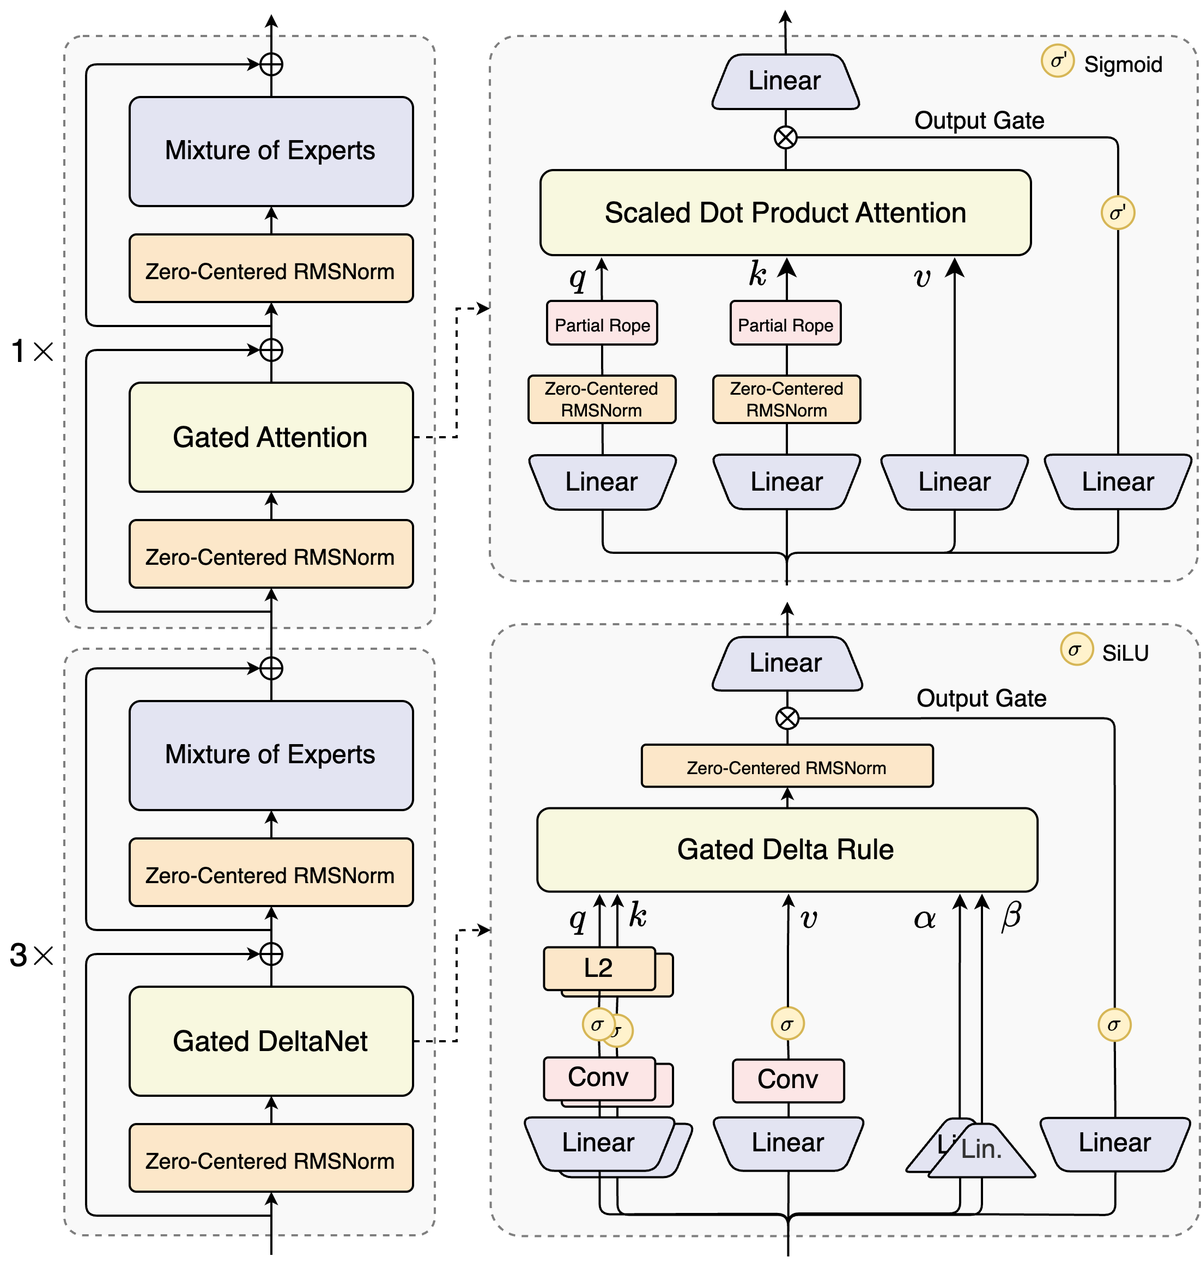
\includegraphics[width=\linewidth,height=.60\textheight,keepaspectratio]{images/Qwen3.8-Flash-Next/fig-21.png}\par{\small Qwen-3.5～Qwen-3.8 架构\par}\end{center}
\end{tcolorbox}
\begin{tcolorbox}[enhanced,blankest,valign=top]
\begin{center}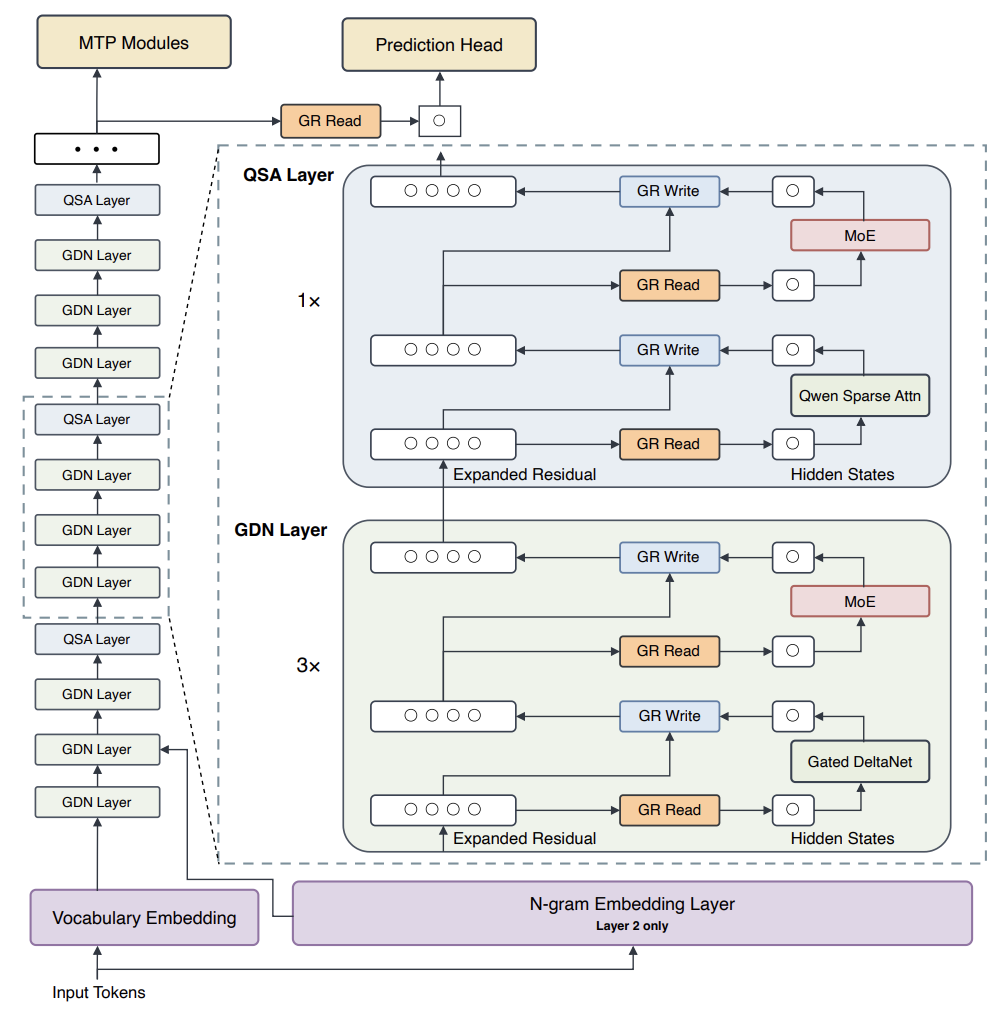
\includegraphics[width=\linewidth,height=.60\textheight,keepaspectratio]{images/Qwen3.8-Flash-Next/fig-23.png}\par{\small Qwen-3.8-next 架构\par}\end{center}
\end{tcolorbox}
\end{tcbraster}
\par\vspace{0.95em}\noindent{\zihao{3}\bfseries \textcolor{feishuBlue}{1.1} 混合架构：GDN（Gated DeltaNet）+ 全注意力}\par\vspace{0.28em}
\begin{tcbraster}[raster columns=2,raster equal height=rows,raster column skip=9pt,raster row skip=8pt,raster left skip=0pt,raster right skip=0pt]
\begin{tcolorbox}[enhanced,blankest,valign=top]
\textcolor{feishuRed}{\textbf{动机：}} 全自注意力和局部注意力存在 trade-off。

\begin{itemize}
\item 全自注意力对每个历史 token 提供直接的、基于内容的访问，代价是计算平方增长、缓存线性增长。
\item 滑动窗口注意力（SWA）把全局访问换成有界的局部感受野，降低了计算和缓存开销，但窗口之外的信息只能靠深度间接传播。
\end{itemize}
\textcolor{feishuRed}{\textbf{实现：}} 全局注意力和局部注意力交错排布，36 层线性注意力 GDN + 12 层全注意力。GDN 把前缀压缩进固定大小的循环状态并按当前内容更新，插在中间的全注意力层保留精确的 token 级检索。

\textcolor{feishuRed}{\textbf{本质上这个排布方式与 }}\textcolor{feishuRed}{\textbf{\href{https://scnajei2ds6y.feishu.cn/wiki/KOBowKTbgiv6ewkHhEBc6qCNnPe}{GLM-5.3-Flash}}}\textcolor{feishuRed}{\textbf{、}}\textcolor{feishuRed}{\textbf{\href{https://scnajei2ds6y.feishu.cn/wiki/Ax5kwJIWRiF7lSkliAucQYwBnHf}{Kimi K3}}}\textcolor{feishuRed}{\textbf{ 的 3:1 混合是同一个逻辑}}：线性层的状态是固定大小的 $d_k\times d_v$ 矩阵，对序列长度不增长，代价是只能保留有损的历史摘要。全注意力保留完整 KV，代价是 $O(L)$ 的缓存。

\end{tcolorbox}
\begin{tcolorbox}[enhanced,blankest,valign=top]
\begin{center}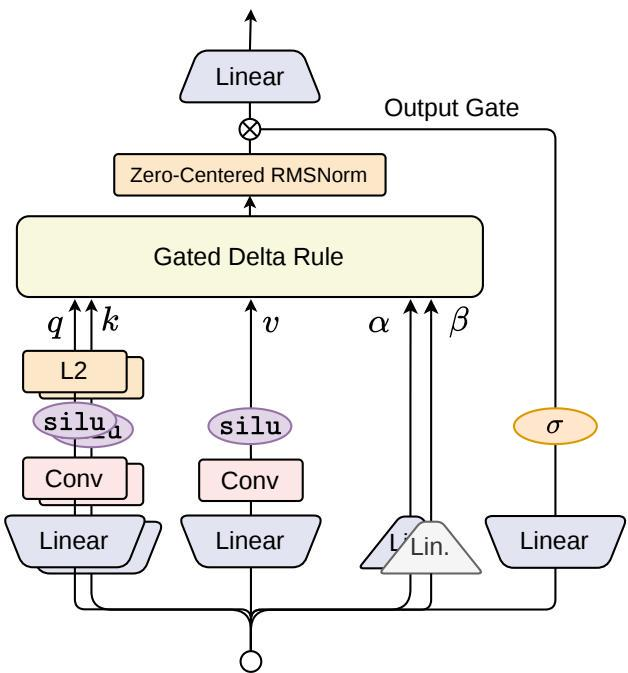
\includegraphics[width=\linewidth,height=.60\textheight,keepaspectratio]{images/Qwen3.8-Flash-Next/fig-33.png}\end{center}
\end{tcolorbox}
\end{tcbraster}
\par\vspace{0.75em}\noindent{\zihao{4}\bfseries \colorbox{headingGreen}{\parbox{\dimexpr\linewidth-2\fboxsep\relax}{\textcolor{feishuBlue}{1.1.1} Gated Delta Rule}}}\par\vspace{0.28em}
线性注意力本质上是维护一个矩阵值循环状态 $\mathbf S_t\in\mathbb R^{d_k\times d_v}$。对每个 head，记 $\mathbf q_t,\mathbf k_t\in\mathbb R^{d_k}$、$\mathbf v_t\in\mathbb R^{d_v}$，GDN 维护状态 $\mathbf S_t\in\mathbb R^{d_k\times d_v}$，施加门控 delta 规则：

\bigmath{\widetilde{\mathbf S}_{t-1}=\alpha_t\mathbf S_{t-1}}
\bigmath{\mathbf e_t=\mathbf v_t-\widetilde{\mathbf S}_{t-1}^{\top}\mathbf k_t}
\bigmath{\mathbf S_t=\widetilde{\mathbf S}_{t-1}+\beta_t\mathbf k_t\mathbf e_t^{\top}}
\bigmath{\mathbf y_t=\mathbf S_t^{\top}\mathbf q_t}
\begin{itemize}
\item $\alpha_t\in(0,1)$ 是数据依赖的标量门，对整个状态矩阵施加统一衰减，作用等价于 $L_2$ 正则（weight decay），每 head 一个标量（代码中 {\setlength{\fboxsep}{0pt}\colorbox{inlinebg}{\strut\ttfamily decay}\colorbox{inlinebg}{\strut\ttfamily \_}\allowbreak{}\colorbox{inlinebg}{\strut\ttfamily t}} 形状为 $[B,H,1,1]$）。
\item $\beta_t\in(0,1)$ 是数据依赖的写入强度，控制本次键值对覆盖旧记忆的幅度，每 head 一个标量。
\item $\mathbf e_t$ 是残差误差：用当前 key 读出已关联的值 $\widetilde{\mathbf S}_{t-1}^{\top}\mathbf k_t$，与真实的 $\mathbf v_t$ 求差。
\end{itemize}
等价地把上面的更新合成一步，得到标准更新表达式：

\bigmath{\mathbf S_t=\alpha_t(I-\beta_t\mathbf k_t\mathbf k_t^{\top})\mathbf S_{t-1}+\beta_t\mathbf k_t\mathbf v_t^{\top}}
\begin{center}\renewcommand{\arraystretch}{1.3}\begin{tabularx}{\linewidth}{|p{1.9cm}|p{1.65cm}|p{.7cm}|>{\raggedright\arraybackslash}X|}
\hline
\rowcolor{tableHead}
方法 & 遗忘门 & delta rule & 更新式（省略归一化）\\\hline
Linear Attention & 无 & 无 & $\mathbf S_t=\mathbf S_{t-1}+\mathbf k_t\mathbf v_t^{\top}$\\\hline
Mamba2 & 数据依赖标量 $\alpha_t$ & 无 & $\mathbf S_t=\alpha_t\mathbf S_{t-1}+\beta_t\mathbf k_t\mathbf v_t^{\top}$\\\hline
GLA & 逐通道 $\operatorname{Diag}(\boldsymbol\alpha_t)$ & 无 & $\mathbf S_t=\operatorname{Diag}(\boldsymbol\alpha_t)\mathbf S_{t-1}+\mathbf k_t\mathbf v_t^{\top}$\\\hline
DeltaNet & 无 & 有 & $\mathbf S_t=(I-\beta_t\mathbf k_t\mathbf k_t^{\top})\mathbf S_{t-1}+\beta_t\mathbf k_t\mathbf v_t^{\top}$\\\hline
GDN & 数据依赖标量 $\alpha_t$ & 有 & $\mathbf S_t=(I-\beta_t\mathbf k_t\mathbf k_t^{\top})\alpha_t\mathbf S_{t-1}+\beta_t\mathbf k_t\mathbf v_t^{\top}$\\\hline
\textcolor{feishuRed}{\textbf{KDA}} & 逐通道 $\operatorname{Diag}(\boldsymbol\alpha_t)$ & 有 & $\mathbf S_t=(I-\beta_t\mathbf k_t\mathbf k_t^{\top})\operatorname{Diag}(\boldsymbol\alpha_t)\mathbf S_{t-1}+\beta_t\mathbf k_t\mathbf v_t^{\top}$\\\hline
\end{tabularx}\end{center}
上面的 4 个更新表达式可以对应到 {\setlength{\fboxsep}{0pt}\colorbox{inlinebg}{\strut\ttfamily torch}\colorbox{inlinebg}{\strut\ttfamily \_}\allowbreak{}\colorbox{inlinebg}{\strut\ttfamily recurrent}\colorbox{inlinebg}{\strut\ttfamily \_}\allowbreak{}\colorbox{inlinebg}{\strut\ttfamily gated}\colorbox{inlinebg}{\strut\ttfamily \_}\allowbreak{}\colorbox{inlinebg}{\strut\ttfamily delta}\colorbox{inlinebg}{\strut\ttfamily \_}\allowbreak{}\colorbox{inlinebg}{\strut\ttfamily rule}} 的解码路径：

\begin{feishuquote}
公式和代码的对应关系：

\begin{itemize}
\item $\alpha_t$ ：{\setlength{\fboxsep}{0pt}\colorbox{inlinebg}{\strut\ttfamily decay}\colorbox{inlinebg}{\strut\ttfamily \_}\allowbreak{}\colorbox{inlinebg}{\strut\ttfamily t}}
\item $\widetilde{\mathbf S}_{t-1}$ ： 乘过 {\setlength{\fboxsep}{0pt}\colorbox{inlinebg}{\strut\ttfamily decay}\colorbox{inlinebg}{\strut\ttfamily \_}\allowbreak{}\colorbox{inlinebg}{\strut\ttfamily t}} 之后的 {\setlength{\fboxsep}{0pt}\colorbox{inlinebg}{\strut\ttfamily last}\colorbox{inlinebg}{\strut\ttfamily \_}\allowbreak{}\colorbox{inlinebg}{\strut\ttfamily recurrent}\colorbox{inlinebg}{\strut\ttfamily \_}\allowbreak{}\colorbox{inlinebg}{\strut\ttfamily state}}
\item $\widetilde{\mathbf S}_{t-1}^{\top}\mathbf k_t$ ： {\setlength{\fboxsep}{0pt}\colorbox{inlinebg}{\strut\ttfamily kv}\colorbox{inlinebg}{\strut\ttfamily \_}\allowbreak{}\colorbox{inlinebg}{\strut\ttfamily mem}}
\item $\beta_t\mathbf e_t$ ： {\setlength{\fboxsep}{0pt}\colorbox{inlinebg}{\strut\ttfamily delta}}
\item $\mathbf y_t$ ： {\setlength{\fboxsep}{0pt}\colorbox{inlinebg}{\strut\ttfamily core}\colorbox{inlinebg}{\strut\ttfamily \_}\allowbreak{}\colorbox{inlinebg}{\strut\ttfamily attn}\colorbox{inlinebg}{\strut\ttfamily \_}\allowbreak{}\colorbox{inlinebg}{\strut\ttfamily out[:,} \colorbox{inlinebg}{\strut\ttfamily :,} \colorbox{inlinebg}{\strut\ttfamily i]}}
\end{itemize}
\end{feishuquote}

\par\vspace{0.75em}\noindent{\zihao{4}\bfseries \colorbox{headingGreen}{\parbox{\dimexpr\linewidth-2\fboxsep\relax}{\textcolor{feishuBlue}{1.1.2} GDN 输入特征处理}}}\par\vspace{0.28em}
内容特征（content features）的参数化用投影加短因果卷积计算：

\bigmath{\begin{aligned}\mathbf q_t&=\operatorname{L2Norm}(\operatorname{SiLU}(\operatorname{ShortConv}(\mathbf W_q\mathbf x_t))),\\\mathbf k_t&=\operatorname{L2Norm}(\operatorname{SiLU}(\operatorname{ShortConv}(\mathbf W_k\mathbf x_t))),\\\mathbf v_t&=\operatorname{SiLU}(\operatorname{ShortConv}(\mathbf W_v\mathbf x_t))\end{aligned}}
写入强度与衰减的计算：

\bigmath{\beta_t=\sigma(\mathbf W_\beta\mathbf x_t),\quad\alpha_t=\exp[-\exp(\mathbf A)\operatorname{softplus}(\mathbf W_\alpha\mathbf x_t+\mathbf b_\alpha)]}
其中 $\mathbf A$ 是每 head 一个的可学习参数，保证 $\alpha_t$ 落在 $(0,1)$。


\par\vspace{0.75em}\noindent{\zihao{4}\bfseries \colorbox{headingGreen}{\parbox{\dimexpr\linewidth-2\fboxsep\relax}{\textcolor{feishuBlue}{1.1.3} GDN 输出门}}}\par\vspace{0.28em}
逐 head 完成递推之后，输出经过归一化，再由一个输入相关的门调制得到输出：

\bigmath{\mathbf o_t=\mathbf W_o[\sigma(\mathbf W_z\mathbf x_t)\odot\operatorname{RMSNorm}(\mathbf y_t)]}
\par\vspace{0.75em}\noindent{\zihao{4}\bfseries \colorbox{headingGreen}{\parbox{\dimexpr\linewidth-2\fboxsep\relax}{\textcolor{feishuBlue}{1.1.4} 全注意力保留 RoPE 位置编码}}}\par\vspace{0.28em}
预训练阶段全注意力层保留 RoPE，理由是：RoPE 和不含位置编码的 NoPE 变体在预训练阶段表现差异不大，然而在后训练后，NoPE 变体会出现显著更高的无限生成现象，因此更容易导致生成无法停止。

\begin{feishubox}{callGreen}{📎}
论文原文：{\setlength{\fboxsep}{0pt}\colorbox{inlinebg}{\strut\ttfamily RoPE} \colorbox{inlinebg}{\strut\ttfamily and} \colorbox{inlinebg}{\strut\ttfamily a} \colorbox{inlinebg}{\strut\ttfamily NoPE} \colorbox{inlinebg}{\strut\ttfamily variant} \colorbox{inlinebg}{\strut\ttfamily without} \colorbox{inlinebg}{\strut\ttfamily positional} \colorbox{inlinebg}{\strut\ttfamily encoding} \colorbox{inlinebg}{\strut\ttfamily show} \colorbox{inlinebg}{\strut\ttfamily little} \colorbox{inlinebg}{\strut\ttfamily difference} \colorbox{inlinebg}{\strut\ttfamily during} \colorbox{inlinebg}{\strut\ttfamily pretraining,} \colorbox{inlinebg}{\strut\ttfamily but} \colorbox{inlinebg}{\strut\ttfamily the} \colorbox{inlinebg}{\strut\ttfamily NoPE} \colorbox{inlinebg}{\strut\ttfamily variant} \colorbox{inlinebg}{\strut\ttfamily exhibits} \colorbox{inlinebg}{\strut\ttfamily a} \colorbox{inlinebg}{\strut\ttfamily substantially} \colorbox{inlinebg}{\strut\ttfamily higher} \colorbox{inlinebg}{\strut\ttfamily rate} \colorbox{inlinebg}{\strut\ttfamily of} \colorbox{inlinebg}{\strut\ttfamily endless} \colorbox{inlinebg}{\strut\ttfamily generation} \colorbox{inlinebg}{\strut\ttfamily after} \colorbox{inlinebg}{\strut\ttfamily post-training} \colorbox{inlinebg}{\strut\ttfamily and} \colorbox{inlinebg}{\strut\ttfamily is} \colorbox{inlinebg}{\strut\ttfamily therefore} \colorbox{inlinebg}{\strut\ttfamily more} \colorbox{inlinebg}{\strut\ttfamily likely} \colorbox{inlinebg}{\strut\ttfamily to} \colorbox{inlinebg}{\strut\ttfamily fail} \colorbox{inlinebg}{\strut\ttfamily to} \colorbox{inlinebg}{\strut\ttfamily terminate.}}

\end{feishubox}

\par\vspace{0.95em}\noindent{\zihao{3}\bfseries \textcolor{feishuBlue}{1.2} QSA（Qwen Sparse Attention）}\par\vspace{0.28em}
\textcolor{feishuRed}{\textbf{动机：}} 稀疏注意力能缓解长上下文下 softmax 注意力的计算复杂度瓶颈。\href{https://my.feishu.cn/wiki/KNFXwJABVitrw7kB3odcnpednXh?larkTabName=space\#share-YjRodvfYnoA4AIxvDVZcBAzPnge}{DSA} （DeepSeek Sparse Attention）用轻量索引器（lightning indexer）生成 token-level 稀疏掩码，\textcolor{feishuRed}{但随着序列变长，索引器自身 }$O(n^2)$\textcolor{feishuRed}{ 的开销不可忽略。}

\textcolor{feishuRed}{\textbf{实现：}} QSA 让索引器先把序列压缩成 micro-block 表示再打分，索引复杂度从 $O(n^2)$ 降到 $O(n^2/r)$。\textcolor{feishuRed}{这与 }\textcolor{feishuRed}{\href{https://scnajei2ds6y.feishu.cn/wiki/KOBowKTbgiv6ewkHhEBc6qCNnPe}{GLM-5.3-Flash}}\textcolor{feishuRed}{ 的 IndexPool 是同一个思路}：都是把细粒度的 token-level 打分改成 block-wise 打分。\textcolor{feishuRed}{区别在压缩方式，IndexPool 用可学习权重的加权池化，QSA 用固定的平均池化。}

\begin{center}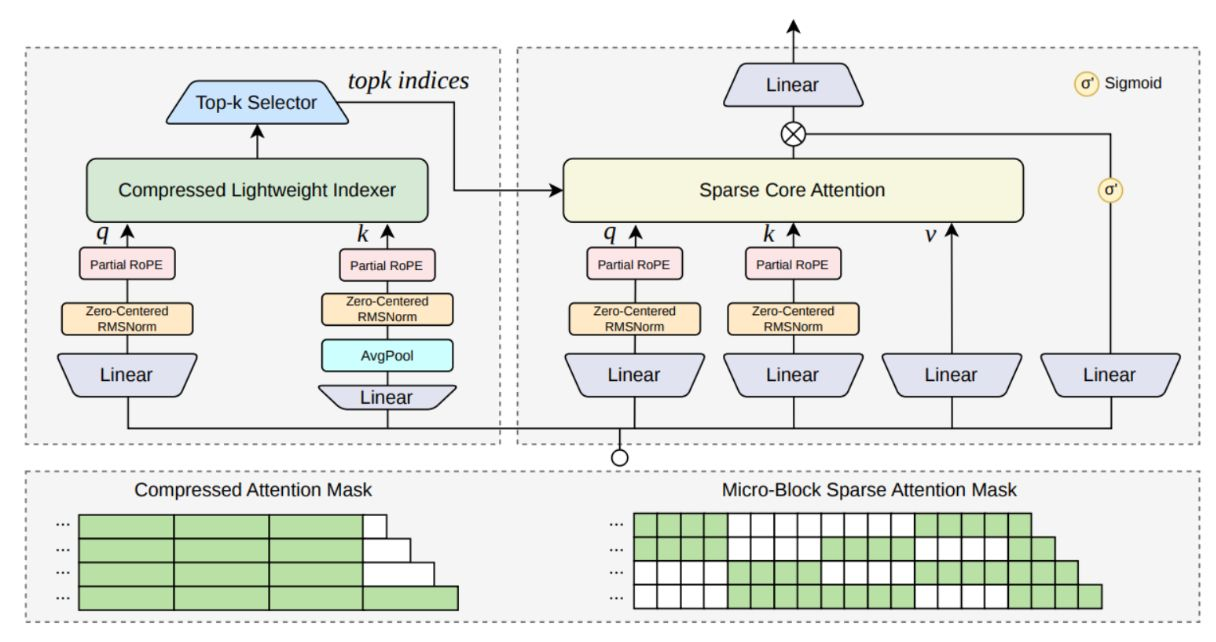
\includegraphics[width=\linewidth,height=.72\textheight,keepaspectratio]{images/Qwen3.8-Flash-Next/fig-94.png}\end{center}
\par\vspace{0.75em}\noindent{\zihao{4}\bfseries \colorbox{headingGreen}{\parbox{\dimexpr\linewidth-2\fboxsep\relax}{\textcolor{feishuBlue}{1.2.1} 压缩索引器（Compressed Lightweight Indexer）}}}\par\vspace{0.28em}
索引器是 MQA 结构，$H$ 个 query head 配一个共享 key head：

\bigmath{\widehat{\mathbf q}_i^h=\operatorname{RMSNorm}(\mathbf W_Q^h\mathbf x_i),\quad\mathbf k_i=\mathbf W_K\mathbf x_i}
$\mathbf W_Q^h$ 是第 $h$ 个 query 头的投影，$\mathbf W_K$ 是共享的 key 投影，$\mathbf x_i$ 是位置 $i$ 的隐状态。

key 按 $r$ 个 token 一组划成互不重叠的块并做平均池化压缩，记块 $b$ 的起始位置为 $p_b=b\cdot r$，再加位置编码：

\bigmath{\widehat{\mathbf k}_b=\operatorname{RMSNorm}(\operatorname{AvgPool}(\mathbf k_{p_b:p_b+r-1})),\quad0\le b<\lfloor n/r\rfloor}
\bigmath{\mathbf q_i^h=\operatorname{PRoPE}(\widehat{\mathbf q}_i^h,i),\quad\bar{\mathbf k}_b=\operatorname{PRoPE}(\widehat{\mathbf k}_b,p_b)}
\begin{itemize}
\item $r$ 是 {\setlength{\fboxsep}{0pt}\colorbox{inlinebg}{\strut\ttfamily indexer}\colorbox{inlinebg}{\strut\ttfamily \_}\allowbreak{}\colorbox{inlinebg}{\strut\ttfamily compress}\colorbox{inlinebg}{\strut\ttfamily \_}\allowbreak{}\colorbox{inlinebg}{\strut\ttfamily ratio}} 取 4。
\item 位置编码用 partial RoPE，只作用在 128 维索引器头的其中 64 维。压缩发生在位置编码之前是为了避免把不同旋转相位的 token 表示平均到一起。
\end{itemize}
\par\vspace{0.75em}\noindent{\zihao{4}\bfseries \colorbox{headingGreen}{\parbox{\dimexpr\linewidth-2\fboxsep\relax}{\textcolor{feishuBlue}{1.2.2} 打分与选择（Scoring and Selection）}}}\par\vspace{0.28em}
Block-wise 重要性分数按 ReLU 激活的 query-key 相似度在索引器头上求和：

\bigmath{I_{ib}=\begin{cases}\sum_{h=1}^{H}\operatorname{ReLU}(\langle\mathbf q_i^h,\bar{\mathbf k}_b\rangle),&p_b+r-1\le i\\-\infty,&\text{otherwise}\end{cases}}
主要注意条件是\textbf{ }\textcolor{feishuRed}{\textbf{block-causal condition}}：query 只能给已被完整观测的块打分。给定 token 预算 $K$，按块预算 $K_B=\lceil K/r\rceil$取 topK，选中的块展开回原始 token 下标，再与最后一个不完整块内的 token 合并（这部分保证被包含）：

\bigmath{\mathcal B_i=\operatorname{TopK}_{K_B}(\{I_{ib}\}_b),\quad\mathcal S_i=\operatorname{Expand}(\mathcal B_i)\cup\{r\lfloor(i+1)/r\rfloor,\ldots,i\}}
\begin{feishubox}{callGreen}{📎}
\textbf{QSA 索引器本质上做的事情：}先把每 4 个 token 的 key 平均成一个块表示，只给块打分、只对块取 top-k，再把选中的块展开回 token。打分量与排序量都因此降到原来的四分之一。

\end{feishubox}
\begin{feishuquote}
\begin{itemize}
\item $\mathbf W_Q^h$ 与 $\mathbf W_K$ ：融合成 {\setlength{\fboxsep}{0pt}\colorbox{inlinebg}{\strut\ttfamily index}\colorbox{inlinebg}{\strut\ttfamily \_}\allowbreak{}\colorbox{inlinebg}{\strut\ttfamily qk}\colorbox{inlinebg}{\strut\ttfamily \_}\allowbreak{}\colorbox{inlinebg}{\strut\ttfamily proj}}，按 {\setlength{\fboxsep}{0pt}\colorbox{inlinebg}{\strut\ttfamily [n}\colorbox{inlinebg}{\strut\ttfamily \_}\allowbreak{}\colorbox{inlinebg}{\strut\ttfamily heads*d,} \colorbox{inlinebg}{\strut\ttfamily kv}\colorbox{inlinebg}{\strut\ttfamily \_}\allowbreak{}\colorbox{inlinebg}{\strut\ttfamily heads*d]}} 切两段。
\item $\widehat{\mathbf q}_i^h$：过完 {\setlength{\fboxsep}{0pt}\colorbox{inlinebg}{\strut\ttfamily q}\colorbox{inlinebg}{\strut\ttfamily \_}\allowbreak{}\colorbox{inlinebg}{\strut\ttfamily layernorm}} 的 {\setlength{\fboxsep}{0pt}\colorbox{inlinebg}{\strut\ttfamily q}}。$\mathbf q_i^h$：再过 {\setlength{\fboxsep}{0pt}\colorbox{inlinebg}{\strut\ttfamily apply}\colorbox{inlinebg}{\strut\ttfamily \_}\allowbreak{}\colorbox{inlinebg}{\strut\ttfamily rotary}\colorbox{inlinebg}{\strut\ttfamily \_}\allowbreak{}\colorbox{inlinebg}{\strut\ttfamily pos}\colorbox{inlinebg}{\strut\ttfamily \_}\allowbreak{}\colorbox{inlinebg}{\strut\ttfamily emb}} 之后的 {\setlength{\fboxsep}{0pt}\colorbox{inlinebg}{\strut\ttfamily q}}。
\item $\mathbf k_i$：{\setlength{\fboxsep}{0pt}\colorbox{inlinebg}{\strut\ttfamily raw}\colorbox{inlinebg}{\strut\ttfamily \_}\allowbreak{}\colorbox{inlinebg}{\strut\ttfamily keys}}。$\widehat{\mathbf k}_b$：{\setlength{\fboxsep}{0pt}\colorbox{inlinebg}{\strut\ttfamily pooled}\colorbox{inlinebg}{\strut\ttfamily \_}\allowbreak{}\colorbox{inlinebg}{\strut\ttfamily keys}}（先 {\setlength{\fboxsep}{0pt}\colorbox{inlinebg}{\strut\ttfamily .mean}} 再 {\setlength{\fboxsep}{0pt}\colorbox{inlinebg}{\strut\ttfamily k}\colorbox{inlinebg}{\strut\ttfamily \_}\allowbreak{}\colorbox{inlinebg}{\strut\ttfamily layernorm}}）。
\item $\bar{\mathbf k}_b$ ：{\setlength{\fboxsep}{0pt}\colorbox{inlinebg}{\strut\ttfamily block}\colorbox{inlinebg}{\strut\ttfamily \_}\allowbreak{}\colorbox{inlinebg}{\strut\ttfamily key}\colorbox{inlinebg}{\strut\ttfamily \_}\allowbreak{}\colorbox{inlinebg}{\strut\ttfamily states}}。$p_b$ ：{\setlength{\fboxsep}{0pt}\colorbox{inlinebg}{\strut\ttfamily group}\colorbox{inlinebg}{\strut\ttfamily \_}\allowbreak{}\colorbox{inlinebg}{\strut\ttfamily starts}}，取每个块内第一个可见 token 的下标。
\item $I_{ib}$：{\setlength{\fboxsep}{0pt}\colorbox{inlinebg}{\strut\ttfamily scores}}。$\mathcal B_i$：{\setlength{\fboxsep}{0pt}\colorbox{inlinebg}{\strut\ttfamily selected}\colorbox{inlinebg}{\strut\ttfamily \_}\allowbreak{}\colorbox{inlinebg}{\strut\ttfamily block}\colorbox{inlinebg}{\strut\ttfamily \_}\allowbreak{}\colorbox{inlinebg}{\strut\ttfamily indices}}。$\mathcal S_i$： {\setlength{\fboxsep}{0pt}\colorbox{inlinebg}{\strut\ttfamily selected}\colorbox{inlinebg}{\strut\ttfamily \_}\allowbreak{}\colorbox{inlinebg}{\strut\ttfamily tokens}}。
\end{itemize}
\end{feishuquote}

\par\vspace{0.75em}\noindent{\zihao{4}\bfseries \colorbox{headingGreen}{\parbox{\dimexpr\linewidth-2\fboxsep\relax}{\textcolor{feishuBlue}{1.2.3} 两阶段蒸馏（Two-stage Distillation）}}}\par\vspace{0.28em}
\href{https://huggingface.co/Qwen/Qwen3.8-Flash-Next}{Qwen/Qwen3.8-Flash-Next} 的 QSA 是在 CPT 阶段引入的，两个阶段都在 256K 序列长度的续训阶段进行。

\begin{itemize}
\item \textcolor{feishuRed}{\textbf{Stage 1：稠密蒸馏（Dense Distillation）：}}把主干的全序列注意力（full-sequence attention）分布蒸馏进索引器（indexer）。Token-level teacher 分布由核心注意力所有头的 softmax 分布求和再做 $L_1$ 归一化，随后用 max pooling 对齐到块级：
\end{itemize}
\bigmath{\begin{aligned}\bar a_{ib}&=\operatorname{MaxPool}(a_{i,p_b:p_b+r-1}),\quad\hat{\mathbf a}_i=\frac{\bar{\mathbf a}_i}{\|\bar{\mathbf a}_i\|_1},\\\mathcal L_{\mathrm{KL}}&=\frac1N\sum_i D_{\mathrm{KL}}(\hat{\mathbf a}_{i,:}\|\operatorname{Softmax}(\mathbf I_{i,:}))\end{aligned}}
\begin{feishubox}{callGreen}{📎}
用 max 而非 mean 聚合的理由是保留显著的 token-level 信号，否则会在聚合时被稀释。

\end{feishubox}
第一阶段只训练索引器（indexer），步数 1000 步，学习率 $1\times10^{-3}$，bs = 8，256K 序列，约 2B token。

\begin{itemize}
\item \textcolor{feishuRed}{\textbf{Stage 2：稀疏训练（Sparse Training）：}}模型主干在索引器（indexer）指导下适应稀疏模式，KL 只在选中的 $K_B$ 个块上计算，且 teacher 概率先在 $\mathcal B_i$ 内重归一化：
\end{itemize}
\bigmath{\mathcal L_{\mathrm{KL}}=\frac1N\sum_iD_{\mathrm{KL}}(\hat{\mathbf a}_{i,\mathcal B_i}\|\operatorname{Softmax}(\mathbf I_{i,\mathcal B_i}))}
第二阶段联合训练 8000 步，学习率 $2.5\times10^{-5}$，bs = 96，256K 序列，约 200B token。


\Needspace{.50\textheight}\par\vspace{0.95em}\noindent{\zihao{3}\bfseries \textcolor{feishuBlue}{1.3} GR（Gated Residual）：门控残差}\par\vspace{0.28em}
\begin{feishuquote}
前置阅读：\href{https://my.feishu.cn/wiki/WsaawrdO3ifrmTk3ab4cSgjBnRb}{mHC：Manifold-Constrained Hyper-Connections}

\end{feishuquote}
\begin{center}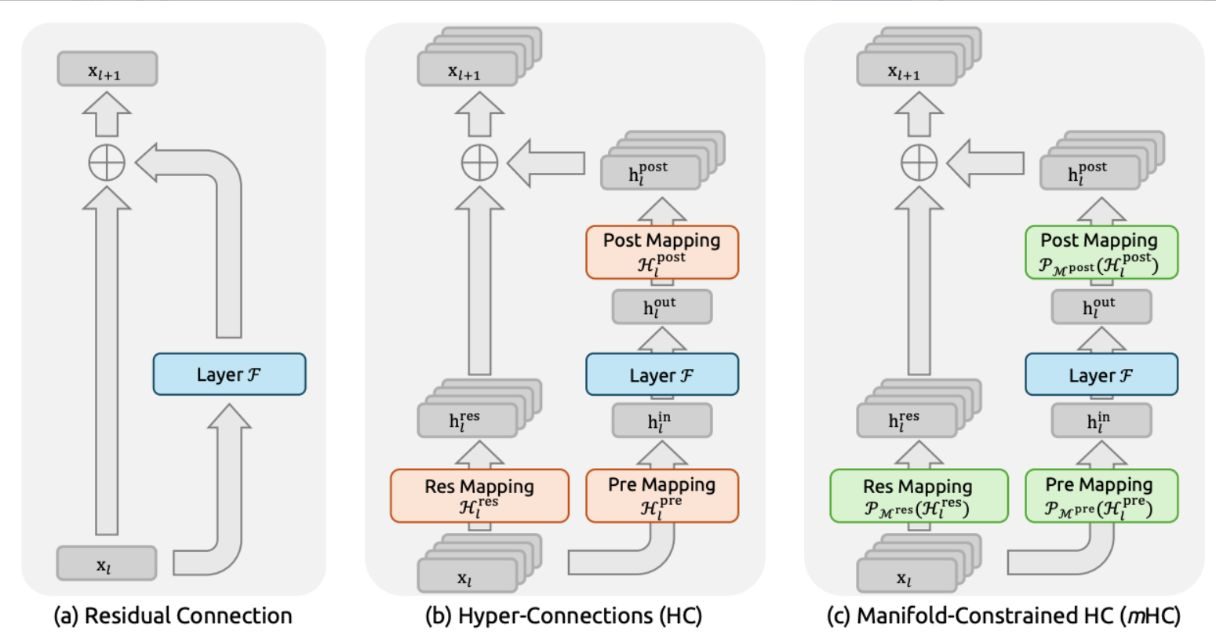
\includegraphics[width=\linewidth,height=.72\textheight,keepaspectratio]{images/Qwen3.8-Flash-Next/fig-125.png}\end{center}
按照\href{https://my.feishu.cn/wiki/WsaawrdO3ifrmTk3ab4cSgjBnRb}{mHC：Manifold-Constrained Hyper-Connections}的逻辑，设$\mathbf x_l\in\mathbb R^{n\times C}$ 是第 $l$ 层的 $n$ 条残差流，残差流从 1 条加宽到 $n$ 条，就有三个操作必须阐明：怎么读（对应映射$\mathcal H_l^{\mathrm{pre}}$）、怎么写（对应映射$\mathcal H_l^{\mathrm{post}}$）、流与流之间混合（对应映射$\mathcal H_l^{\mathrm{res}}$）。 HC、mHC、GR 本质区别就在这三个操作的设计上。

\par\vspace{0.75em}\noindent{\zihao{4}\bfseries \colorbox{headingGreen}{\parbox{\dimexpr\linewidth-2\fboxsep\relax}{\textcolor{feishuBlue}{1.3.1} 回顾 HC 与 mHC}}}\par\vspace{0.28em}
标准残差只有单流，等价于恒等读、恒等写、恒等混合：

\bigmath{\mathbf x_{l+1}=\mathbf x_l+\mathcal F(\mathbf x_l,\mathbf W_l)}
HC 把流加宽成 $n$ 条，并把上面三个操作设置分别为三个可学习映射算子：

\bigmath{\mathbf x_{l+1}=\mathcal H_l^{\mathrm{res}}\mathbf x_l+\mathcal H_l^{\mathrm{post}\top}\mathcal F(\mathcal H_l^{\mathrm{pre}}\mathbf x_l,\mathbf W_l)}
\begin{itemize}
\item $\mathcal H_l^{\mathrm{pre}}\in\mathbb R^{1\times n}$ 是\textcolor{feishuRed}{\textbf{读操作}}：$n$ 个标量，把 $n$ 条流加权成 1 条 $C$ 维向量送进子层 $\mathcal F$。
\item $\mathcal H_l^{\mathrm{post}}\in\mathbb R^{1\times n}$ 是\textcolor{feishuRed}{\textbf{写操作}}：$n$ 个标量，把子层的 1 条输出展开写回 $n$ 条流。
\item $\mathcal H_l^{\mathrm{res}}\in\mathbb R^{n\times n}$ 是\textcolor{feishuRed}{\textbf{混合操作}}：让第 $i$ 条流的新值含第 $j$ 条流的成分。
\end{itemize}
把上面的 HC 表达式递推展开从第 $l$层到第 $L$ 层：

\bigmath{\begin{aligned}\mathbf x_L={}&\left(\prod_{i=1}^{L-l}\mathcal H_{L-i}^{\mathrm{res}}\right)\mathbf x_l\\&+\sum_{i=l}^{L-1}\left(\prod_{j=1}^{L-1-i}\mathcal H_{L-j}^{\mathrm{res}}\right)\mathcal H_i^{\mathrm{post}\top}\mathcal F(\mathcal H_i^{\mathrm{pre}}\mathbf x_i,\mathbf W_i)\end{aligned}}
其中$\prod_{i=1}^{L-l}\mathcal H_{L-i}^{\mathrm{res}}$ 是 residual stream 的复合残差映射（composite mapping）

\textcolor{feishuRed}{问题在于：}$\mathcal H_l^{\mathrm{res}}$\textcolor{feishuRed}{ 是无约束可学习矩阵，多层连乘 }$\prod_{i=1}^{L-l}\mathcal H_{L-i}^{\mathrm{res}}$\textcolor{feishuRed}{ 极容易发生梯度爆炸或消失。}或者说复合映射是无约束的，在层数增加后会愈发偏离 identity mapping。论文里用 Amax Gain Magnitude 量化了这一过程：

\begin{itemize}
\item Forward：复合映射的最大行绝对和（最大行和），衡量前向传播的信号放大倍数。
\item Backward：复合映射的最大列绝对和（最大列和），衡量反向传播的梯度放大倍数。
\end{itemize}
通过27B模型的训练消融，可以得出：单层映射 $\mathcal H_l^{\mathrm{res}}$ 的 Amax Gain Magnitude 理想情况接近 1。复合映射 $\prod_{i=1}^{L-l}\mathcal H_{L-i}^{\mathrm{res}}$ 的峰值接近 3000>>1，直接导致了训练不稳定。对应的，训练在 12k step 左右出现明显的 loss spike 和 gradient norm 爆炸：

\begin{tcbraster}[raster columns=2,raster equal height=rows,raster column skip=9pt,raster row skip=8pt,raster left skip=0pt,raster right skip=0pt]
\begin{tcolorbox}[enhanced,blankest,valign=top]
\begin{center}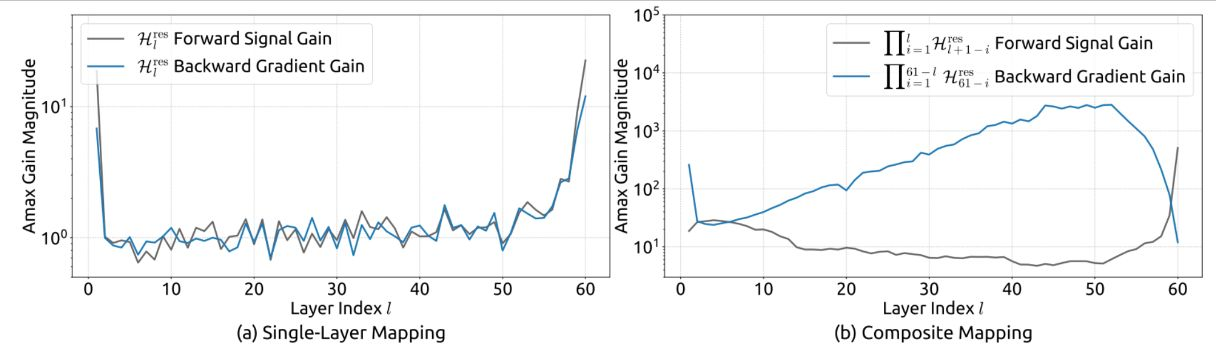
\includegraphics[width=\linewidth,height=.60\textheight,keepaspectratio]{images/Qwen3.8-Flash-Next/fig-283.png}\end{center}
\end{tcolorbox}
\begin{tcolorbox}[enhanced,blankest,valign=top]
\begin{center}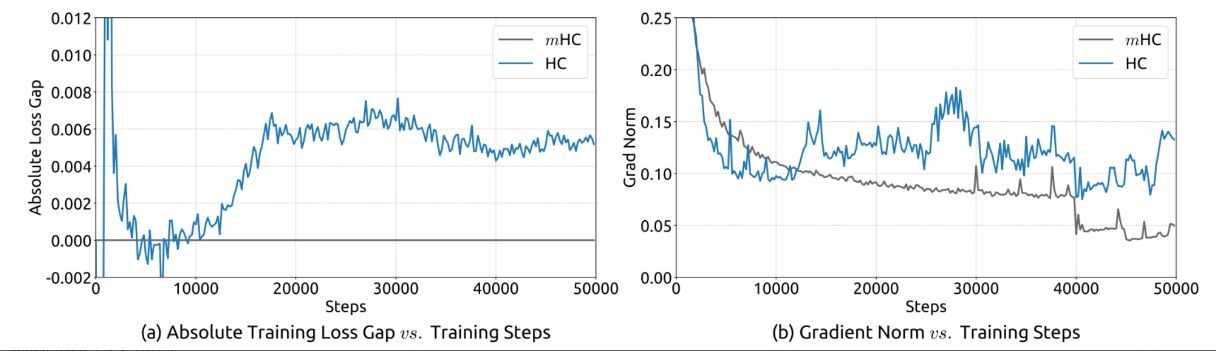
\includegraphics[width=\linewidth,height=.60\textheight,keepaspectratio]{images/Qwen3.8-Flash-Next/fig-285.png}\end{center}
\end{tcolorbox}
\end{tcbraster}
mHC 的解法是保留 $\mathcal H_l^{\mathrm{res}}$、把它约束到双随机矩阵流形上（每行和、每列和都为 1，元素非负），用 20 轮 Sinkhorn-Knopp 迭代投影。双随机矩阵谱范数不超过 1 且对乘法封闭，连乘项因此不再放大信号。代价是每层多 20 轮迭代，而且残差流宽 $n$ 倍带来的访存开销并没有解决。


\par\vspace{0.75em}\noindent{\zihao{4}\bfseries \colorbox{headingGreen}{\parbox{\dimexpr\linewidth-2\fboxsep\relax}{\textcolor{feishuBlue}{1.3.2} GR 的解法：去除多流混合}}}\par\vspace{0.28em}
Qwen-3.8-Next 通过消融认为$\mathcal H_l^{\mathrm{res}}$带来的增益有限：$\mathcal H^{\mathrm{res}}$ adds little. Once the read and the write are expressive enough, adding the $n_r\times n_r$ mixing operator brings no significant improvement.

因此 GR 直接去掉混合算子，更新式：

\bigmath{\mathbf x_{l+1}=\mathbf x_l+\mathcal H_l^{\mathrm{post}\top}\mathcal F\!\left(\frac1n\sum_{i=1}^n\mathcal H_{l,i}^{\mathrm{pre}}\odot\widetilde{\mathbf x}_{l,i},\,\mathbf W_l\right)}
\textbf{对比以上 HC 的更新式的区别：}

\begin{enumerate}
\item[\textcolor{feishuBlue}{1.}] 残差项从 $\mathcal H_l^{\mathrm{res}}\mathbf x_l$ 退化成 $\mathbf x_l$，可以看作 $\mathcal H_l^{\mathrm{res}}$ 被单位矩阵取代。因此去除了递推展开连乘项，也就不需要 mHC 的双随机流形与 Sinkhorn 迭代。
\item[\textcolor{feishuBlue}{2.}] 读从矩阵乘变成逐元素乘 $\odot$，因为 $\mathcal H_l^{\mathrm{pre}}$ 的形状从 $1\times n$ 拓展为 $n\times C$，同时 $\widetilde{\mathbf x}_l$ 为原始的 $\mathbf x_l$的归一化。
\end{enumerate}
\textcolor{feishuRed}{\textbf{完整的 GR 计算流程：}}

\begin{enumerate}
\item 先把 $n$ 条流独立归一化：
\bigmath{\widetilde{\mathbf x}_{l,i}=\operatorname{RMSNorm}(\mathbf x_{l,i};\boldsymbol\gamma_i),\quad i=1,\ldots,n}
$\mathbf x_{l,i}\in\mathbb R^C$ 是第 $i$ 条流，$\boldsymbol\gamma_i\in\mathbb R^C$ 是第 $i$ 条流独立的可学习缩放。

\begin{feishubox}{callGreen}{🧭}
与 mHC 的区别：mHC 是先 $\operatorname{vec}(\mathbf x_l)$ 拼成 $1\times nC$ 再整体做一次 RMSNorm。GR 是 $n$ 条流独立归一化，各自维护可学习缩放 $\boldsymbol\gamma_i$。

\end{feishubox}
\item 从拼接 $\operatorname{vec}(\widetilde{\mathbf x}_l)\in\mathbb R^{nC}$ 计算出读、写变换：
\bigmath{\mathcal H_l^{\mathrm{pre}}=\operatorname{unvec}\sigma\!\left(\mathbf W_u\operatorname{SiLU}\!\left(\frac1n\mathbf W_d\operatorname{vec}(\widetilde{\mathbf x}_l)\right)\right)\in\mathbb R^{n\times C}}
\bigmath{\mathcal H_l^{\mathrm{post}}=2\sigma\!\left(\frac1n\mathbf W_w\operatorname{vec}(\widetilde{\mathbf x}_l)\right)\in\mathbb R^n}
\begin{itemize}
\item $\mathbf W_d\in\mathbb R^{r\times nC}$ 把 $nC=4\times2560=10240$ 维压到 low-rank 维度 $r$，$\mathbf W_u\in\mathbb R^{nC\times r}$ 再升回 10240 维。 low-rank 维度 $r=C/8=320$，即配置里的 {\setlength{\fboxsep}{0pt}\colorbox{inlinebg}{\strut\ttfamily hc}\colorbox{inlinebg}{\strut\ttfamily \_}\allowbreak{}\colorbox{inlinebg}{\strut\ttfamily lowrank}}，目的是压缩参数量（相比$10240^2$ 满秩矩阵变换）。
\item $\mathbf W_w\in\mathbb R^{n\times nC}$ 即 $[4,10240]$，计算 4 个分流系数。
\item $\sigma$ 是 Sigmoid，$\operatorname{unvec}$ 把 10240 维 reshape 为 $n\times C$。
\end{itemize}
\item 使用更新式进行计算：$\mathbf x_{l+1}=\mathbf x_l+\mathcal H_l^{\mathrm{post}\top}\mathcal F\!\left(\frac1n\sum_{i=1}^n\mathcal H_{l,i}^{\mathrm{pre}}\odot\widetilde{\mathbf x}_{l,i},\,\mathbf W_l\right)$
\begin{feishubox}{callGreen}{🧭}
\textcolor{feishuRed}{\textbf{在三个操作上， GR 与 mHC 对比：}}

\begin{itemize}
\item $\mathcal H_l^{\mathrm{pre}}$：mHC 是 $\sigma(\cdot)\in\mathbb R^{1\times n}$，$n$ 个权重标量。GR 是 $\sigma(\cdot)\in\mathbb R^{n\times C}$，$n\times C$ 个门控标量。
\item $\mathcal H_l^{\mathrm{post}}$：两边都是 $2\sigma(\cdot)$，形式一致。
\item $\mathcal H_l^{\mathrm{res}}$：mHC 是 $\operatorname{Sinkhorn}(\cdot)\in\mathbb R^{n\times n}$。GR 去除这个操作（恒等变换）。
\end{itemize}
以上操作对应 GR 的消融结论，读的粒度比写的粒度重要，同样的细化施加在写上几乎没有收益，因此施加逐元素（element-wise）的门控（gating）。代码实现逻辑参考以下代码：

\end{feishubox}
\begin{feishuquote}
\begin{itemize}
\item $\mathbf x_l$ ：{\setlength{\fboxsep}{0pt}\colorbox{inlinebg}{\strut\ttfamily hyper}\colorbox{inlinebg}{\strut\ttfamily \_}\allowbreak{}\colorbox{inlinebg}{\strut\ttfamily input}}，$\widetilde{\mathbf x}_l$： {\setlength{\fboxsep}{0pt}\colorbox{inlinebg}{\strut\ttfamily hyper}\colorbox{inlinebg}{\strut\ttfamily \_}\allowbreak{}\colorbox{inlinebg}{\strut\ttfamily input}\colorbox{inlinebg}{\strut\ttfamily \_}\allowbreak{}\colorbox{inlinebg}{\strut\ttfamily normed}}。
\item $\boldsymbol\gamma_i$ ：{\setlength{\fboxsep}{0pt}\colorbox{inlinebg}{\strut\ttfamily hc}\colorbox{inlinebg}{\strut\ttfamily \_}\allowbreak{}\colorbox{inlinebg}{\strut\ttfamily norm.weight}} 的第 $i$ 段。
\item $\mathbf W_d$ ： {\setlength{\fboxsep}{0pt}\colorbox{inlinebg}{\strut\ttfamily input}\colorbox{inlinebg}{\strut\ttfamily \_}\allowbreak{}\colorbox{inlinebg}{\strut\ttfamily mix}\colorbox{inlinebg}{\strut\ttfamily \_}\allowbreak{}\colorbox{inlinebg}{\strut\ttfamily weight}\colorbox{inlinebg}{\strut\ttfamily \_}\allowbreak{}\colorbox{inlinebg}{\strut\ttfamily down}}，$\mathbf W_u$： {\setlength{\fboxsep}{0pt}\colorbox{inlinebg}{\strut\ttfamily input}\colorbox{inlinebg}{\strut\ttfamily \_}\allowbreak{}\colorbox{inlinebg}{\strut\ttfamily mix}\colorbox{inlinebg}{\strut\ttfamily \_}\allowbreak{}\colorbox{inlinebg}{\strut\ttfamily weight}\colorbox{inlinebg}{\strut\ttfamily \_}\allowbreak{}\colorbox{inlinebg}{\strut\ttfamily up}}，$\mathbf W_w$ 对应 {\setlength{\fboxsep}{0pt}\colorbox{inlinebg}{\strut\ttfamily block}\colorbox{inlinebg}{\strut\ttfamily \_}\allowbreak{}\colorbox{inlinebg}{\strut\ttfamily inject}\colorbox{inlinebg}{\strut\ttfamily \_}\allowbreak{}\colorbox{inlinebg}{\strut\ttfamily weight}}。
\item $\mathcal H_l^{\mathrm{pre}}$： {\setlength{\fboxsep}{0pt}\colorbox{inlinebg}{\strut\ttfamily unflatten}} 之后的 {\setlength{\fboxsep}{0pt}\colorbox{inlinebg}{\strut\ttfamily input}\colorbox{inlinebg}{\strut\ttfamily \_}\allowbreak{}\colorbox{inlinebg}{\strut\ttfamily mix}\colorbox{inlinebg}{\strut\ttfamily \_}\allowbreak{}\colorbox{inlinebg}{\strut\ttfamily weight}}，$\mathcal H_l^{\mathrm{post}}$：{\setlength{\fboxsep}{0pt}\colorbox{inlinebg}{\strut\ttfamily injection}\colorbox{inlinebg}{\strut\ttfamily \_}\allowbreak{}\colorbox{inlinebg}{\strut\ttfamily weights}}。
\end{itemize}
\end{feishuquote}
\end{enumerate}

\par\vspace{0.75em}\noindent{\zihao{4}\bfseries \colorbox{headingGreen}{\parbox{\dimexpr\linewidth-2\fboxsep\relax}{\textcolor{feishuBlue}{1.3.3} GatedNorm 替代 Pre-Norm}}}\par\vspace{0.28em}
\begin{tcbraster}[raster columns=2,raster equal height=rows,raster column skip=9pt,raster row skip=8pt,raster left skip=0pt,raster right skip=0pt]
\begin{tcolorbox}[enhanced,blankest,valign=top]
\begin{center}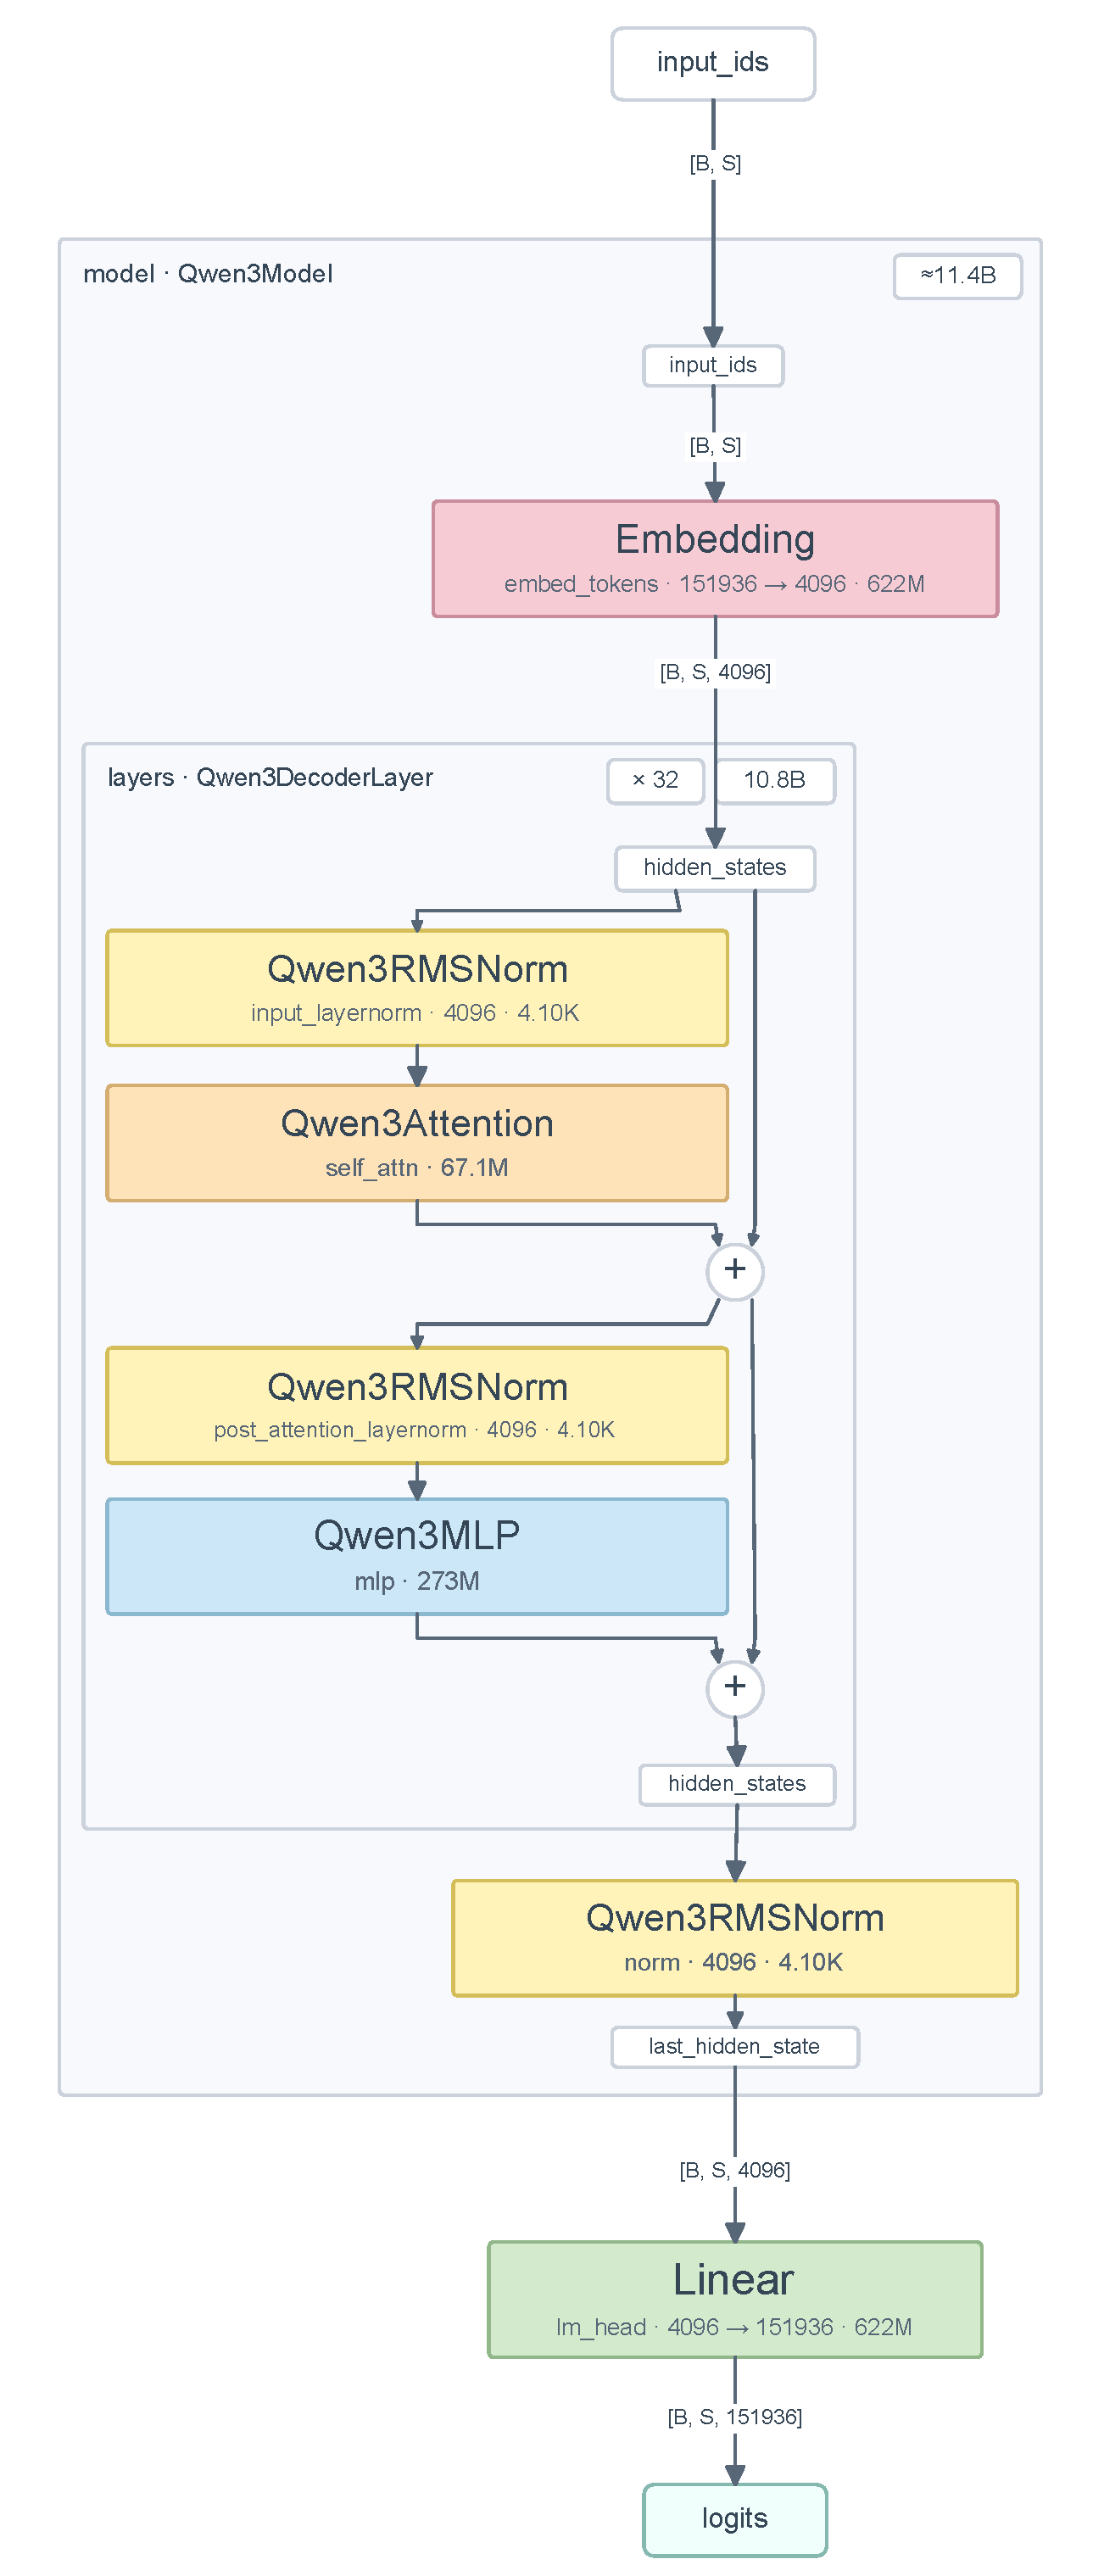
\includegraphics[width=\linewidth,height=.60\textheight,keepaspectratio]{images/Qwen3.8-Flash-Next/redraw/exports/fig-297.pdf}\par{\small Qwen-3 Pre-Norm 示例\par}\end{center}
\end{tcolorbox}
\begin{tcolorbox}[enhanced,blankest,valign=top]
\begin{center}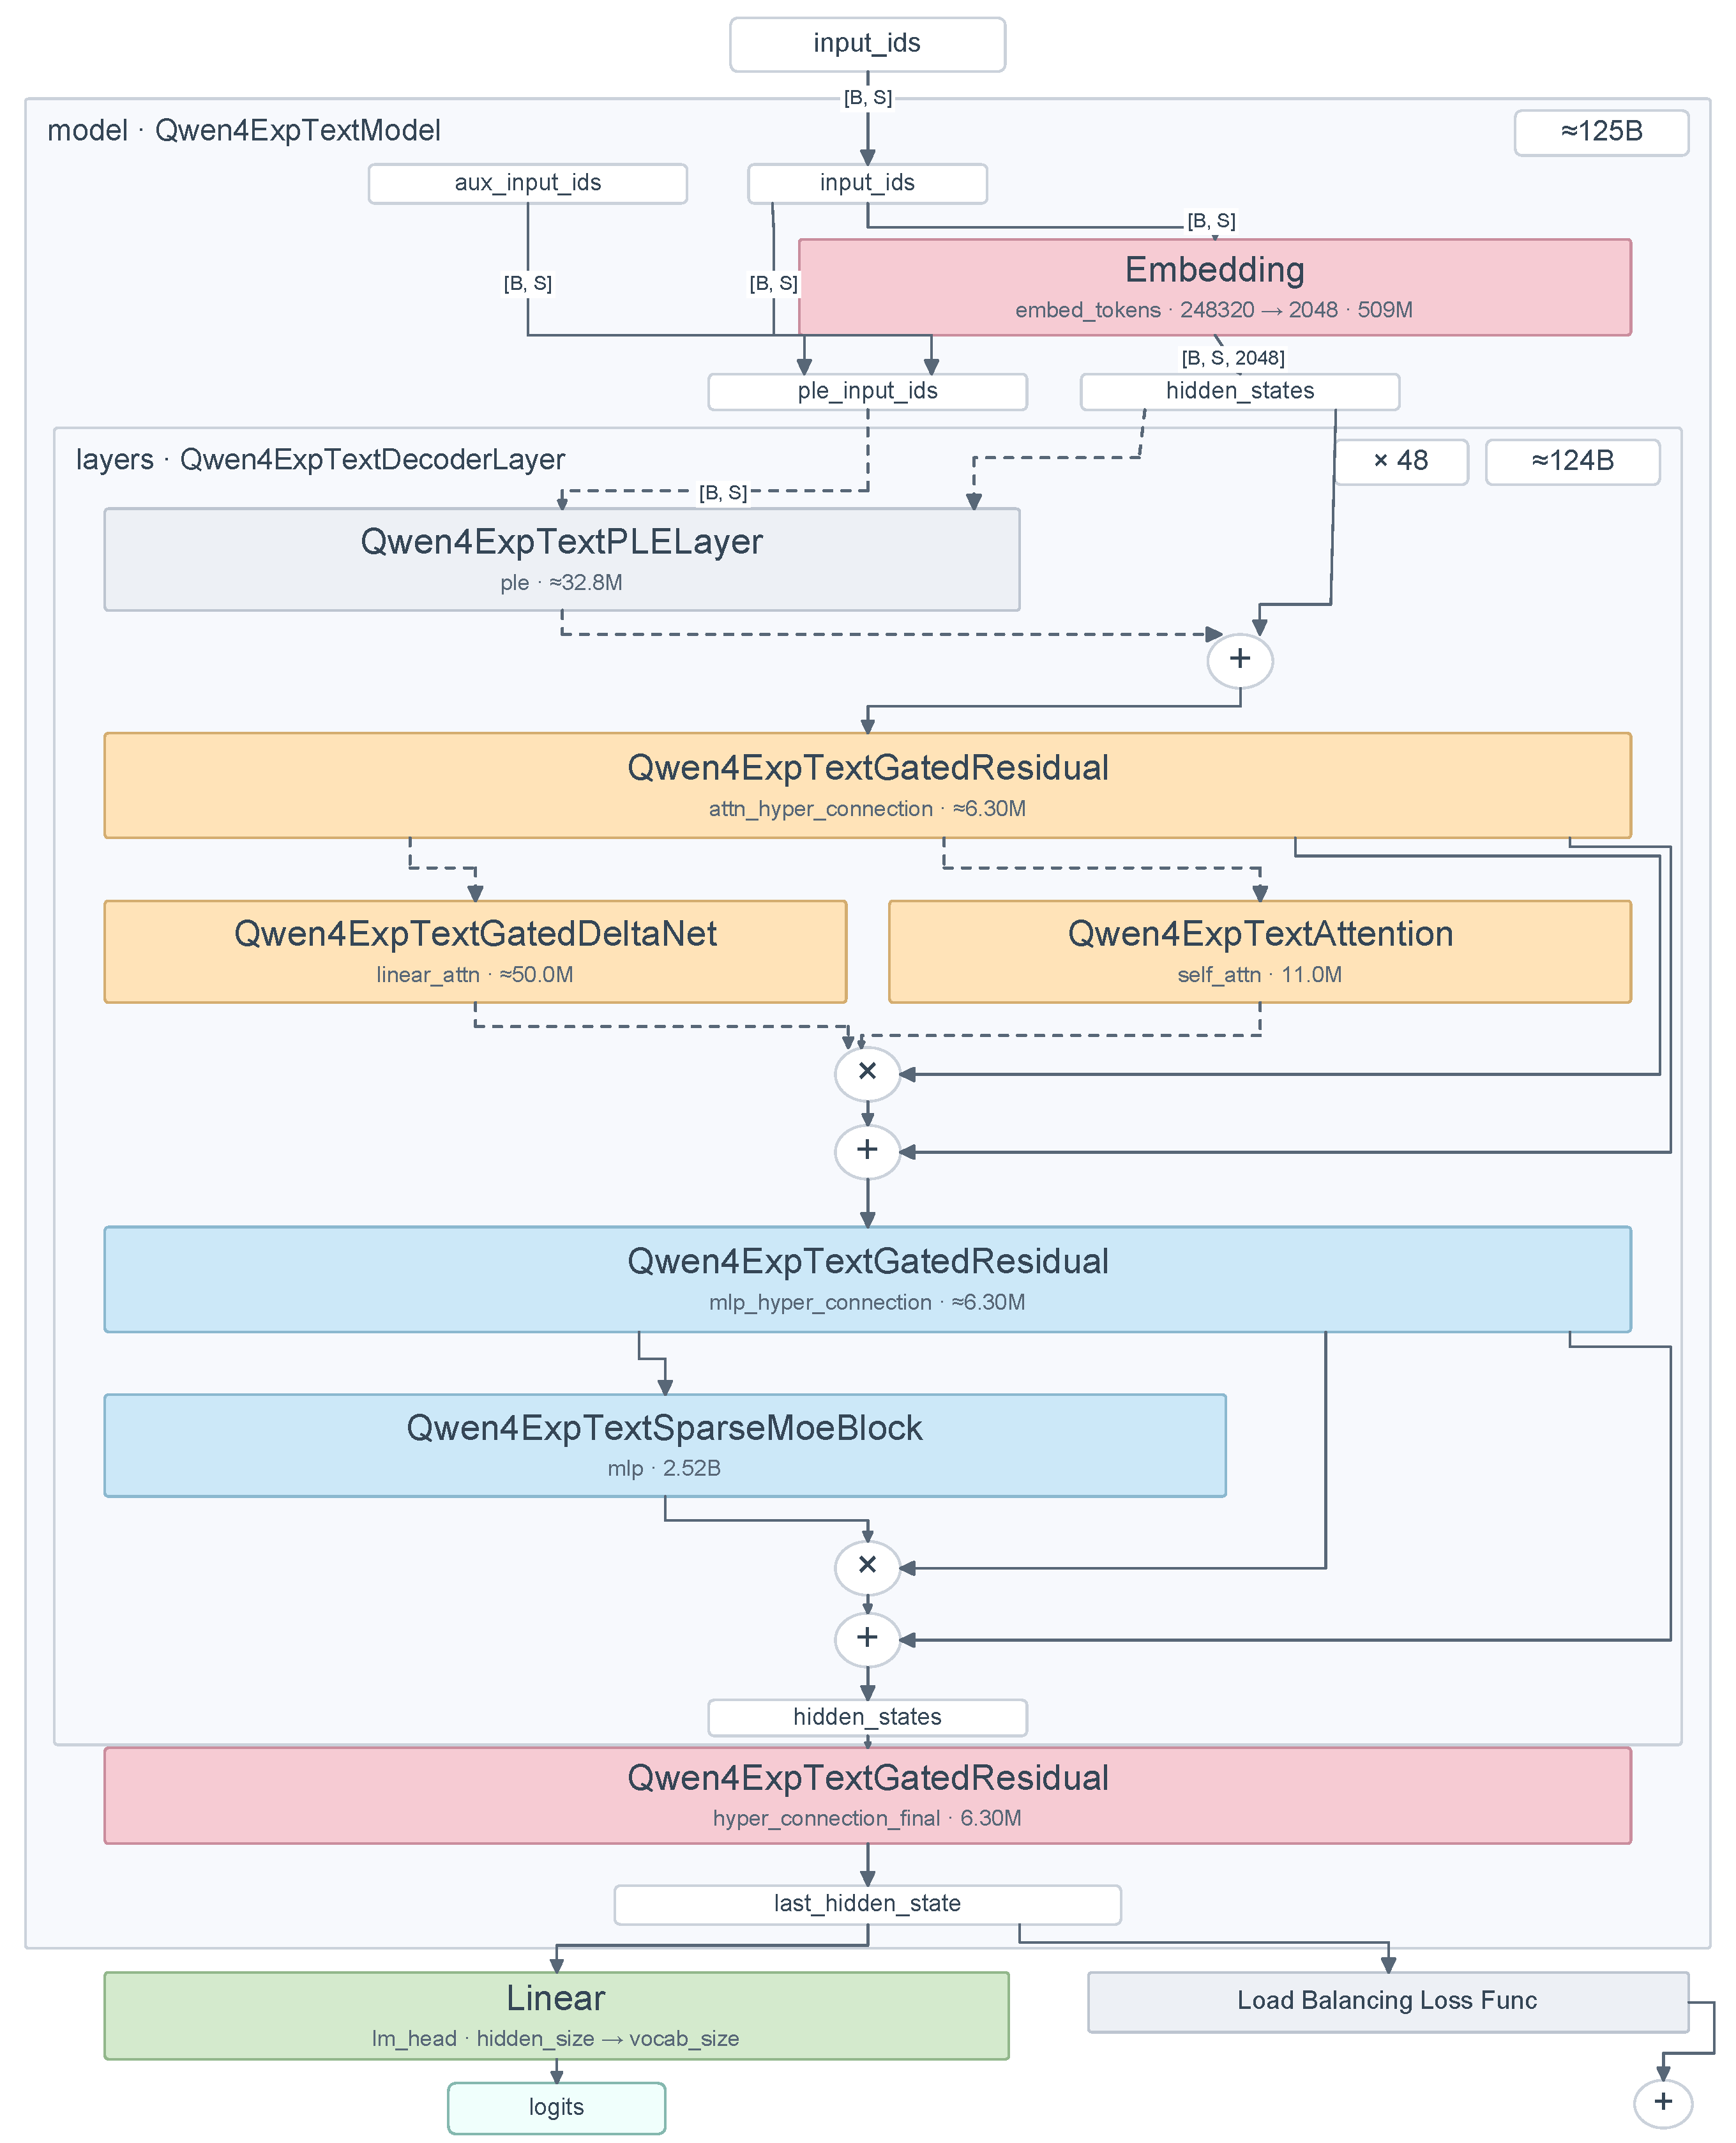
\includegraphics[width=\linewidth,height=.60\textheight,keepaspectratio]{images/Qwen3.8-Flash-Next/redraw/exports/fig-299.pdf}\par{\small Qwen-3.8-Next GatedNorm 替代 Pre-Norm\par}\end{center}
\begin{center}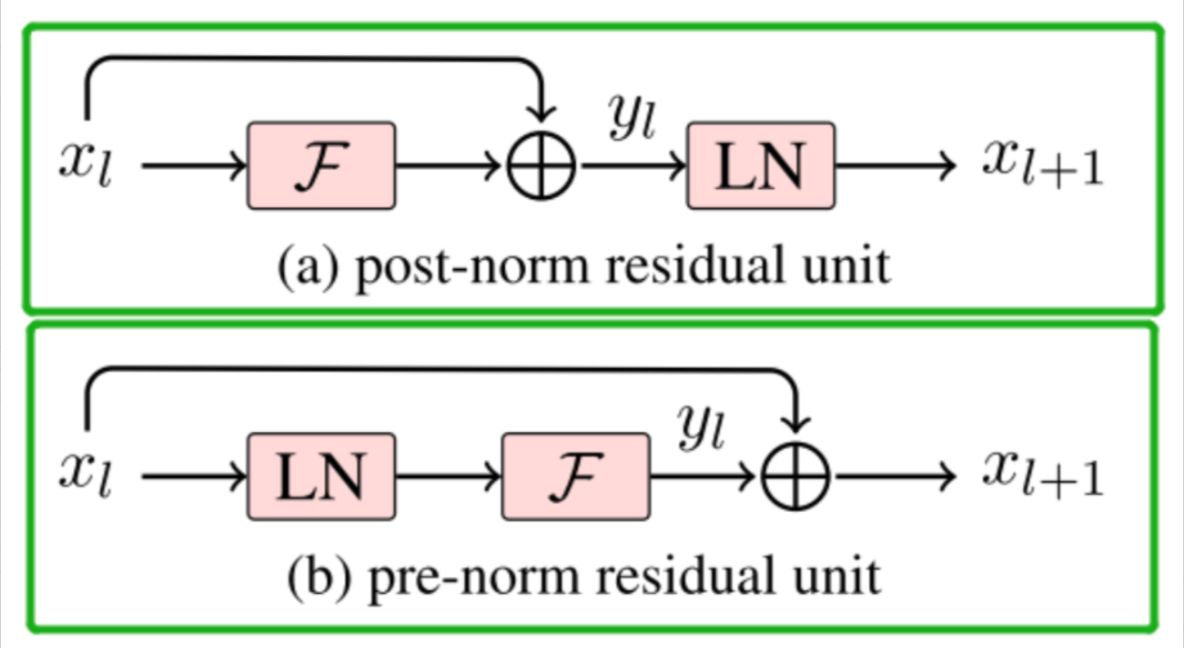
\includegraphics[width=\linewidth,height=.60\textheight,keepaspectratio]{images/Qwen3.8-Flash-Next/fig-300.png}\par{\small Pre-Norm\textbackslash{}Post-Norm 对比\par}\end{center}
\end{tcolorbox}
\end{tcbraster}
在前序工作\href{https://arxiv.org/pdf/2601.22966}{《A Unified View of Attention and Residual Sinks: Outlier-Driven Rescaling is Essential for Transformer Training》}中有结论：

在 RMSNorm 之后加一个轻量的逐元素门可显著改善训练稳定性，即 GatedNorm，公式表达为：

\bigmath{\operatorname{GatedNorm}(\mathbf u)=\operatorname{RMSNorm}(\mathbf u)\odot\sigma(\mathbf W_2\operatorname{SiLU}(\mathbf W_1\operatorname{RMSNorm}(\mathbf u)))}
其中 $\mathbf W_1$ 与 $\mathbf W_2$ 是一对低秩投影，先降维再升回原维度。

把这个表达式与上面 GR 的 $\mathcal H_l^{\mathrm{pre}}$ 更新式对比，本质上两者是同一个结构：归一化、低秩降维、SiLU、升维、Sigmoid、再逐元素乘，区别仅在于 GatedNorm 作用于单流，GR 的读作用于 $n$ 条流拼起来的向量。

因此 Qwen-3.8-Next 将两者合并成一个算子：GR 的读已经包含归一化与门控，所以它取代了子层的预归一化（Pre-Norm），参考上图可以清晰看出这个结构。

还有一个需要注意的细节是 n（n=4）条流的进出口（如何从单流进行拓展），N 流的入口状态来自 {\setlength{\fboxsep}{0pt}\colorbox{inlinebg}{\strut\ttfamily repeat}} 而不是 $n$ 组独立初始化：


\par\vspace{0.95em}\noindent{\zihao{3}\bfseries \textcolor{feishuBlue}{1.4} N-gram Embedding}\par\vspace{0.28em}
\begin{feishuquote}
前置阅读 \href{https://my.feishu.cn/wiki/JwXTw0oUeimyoBk2QIgcSfBfn9g}{Engram：Conditional Memory via Scalable Lookup}：通过 Embedding 进行模型的记忆扩容。

\end{feishuquote}
\begin{tcbraster}[raster columns=2,raster equal height=rows,raster column skip=9pt,raster row skip=8pt,raster left skip=0pt,raster right skip=0pt]
\begin{tcolorbox}[enhanced,blankest,valign=top]
\begin{feishuboxnb}{callGreen}{🧭}
N-gram Embedding 把当前 token id（unigram）为 key 查表推广为以局部上下文（n-gram）为查表的 key：以每个 token 结尾的 n-gram 作为 Key 查表，取回的向量增强该 token 的表示。

这个做法的优点是在几乎不增加逐 token FLOPs 的前提下进行记忆扩容，并且使用主机内存卸载与异步预取进行确定性寻址。

\end{feishuboxnb}
\end{tcolorbox}
\begin{tcolorbox}[enhanced,blankest,valign=top]
\begin{center}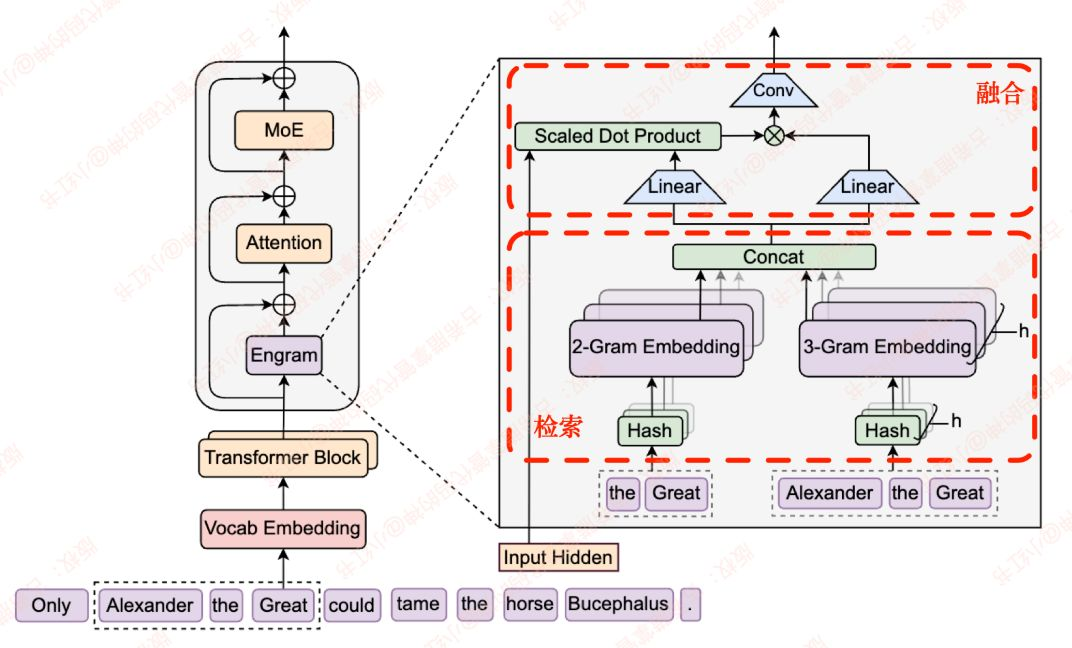
\includegraphics[width=\linewidth,height=.60\textheight,keepaspectratio]{images/Qwen3.8-Flash-Next/fig-307.png}\par{\small Engram 架构示意图\par}\end{center}
\end{tcolorbox}
\end{tcbraster}
\Needspace{.70\textheight}
\begin{center}
\begin{minipage}{\linewidth}
\centering
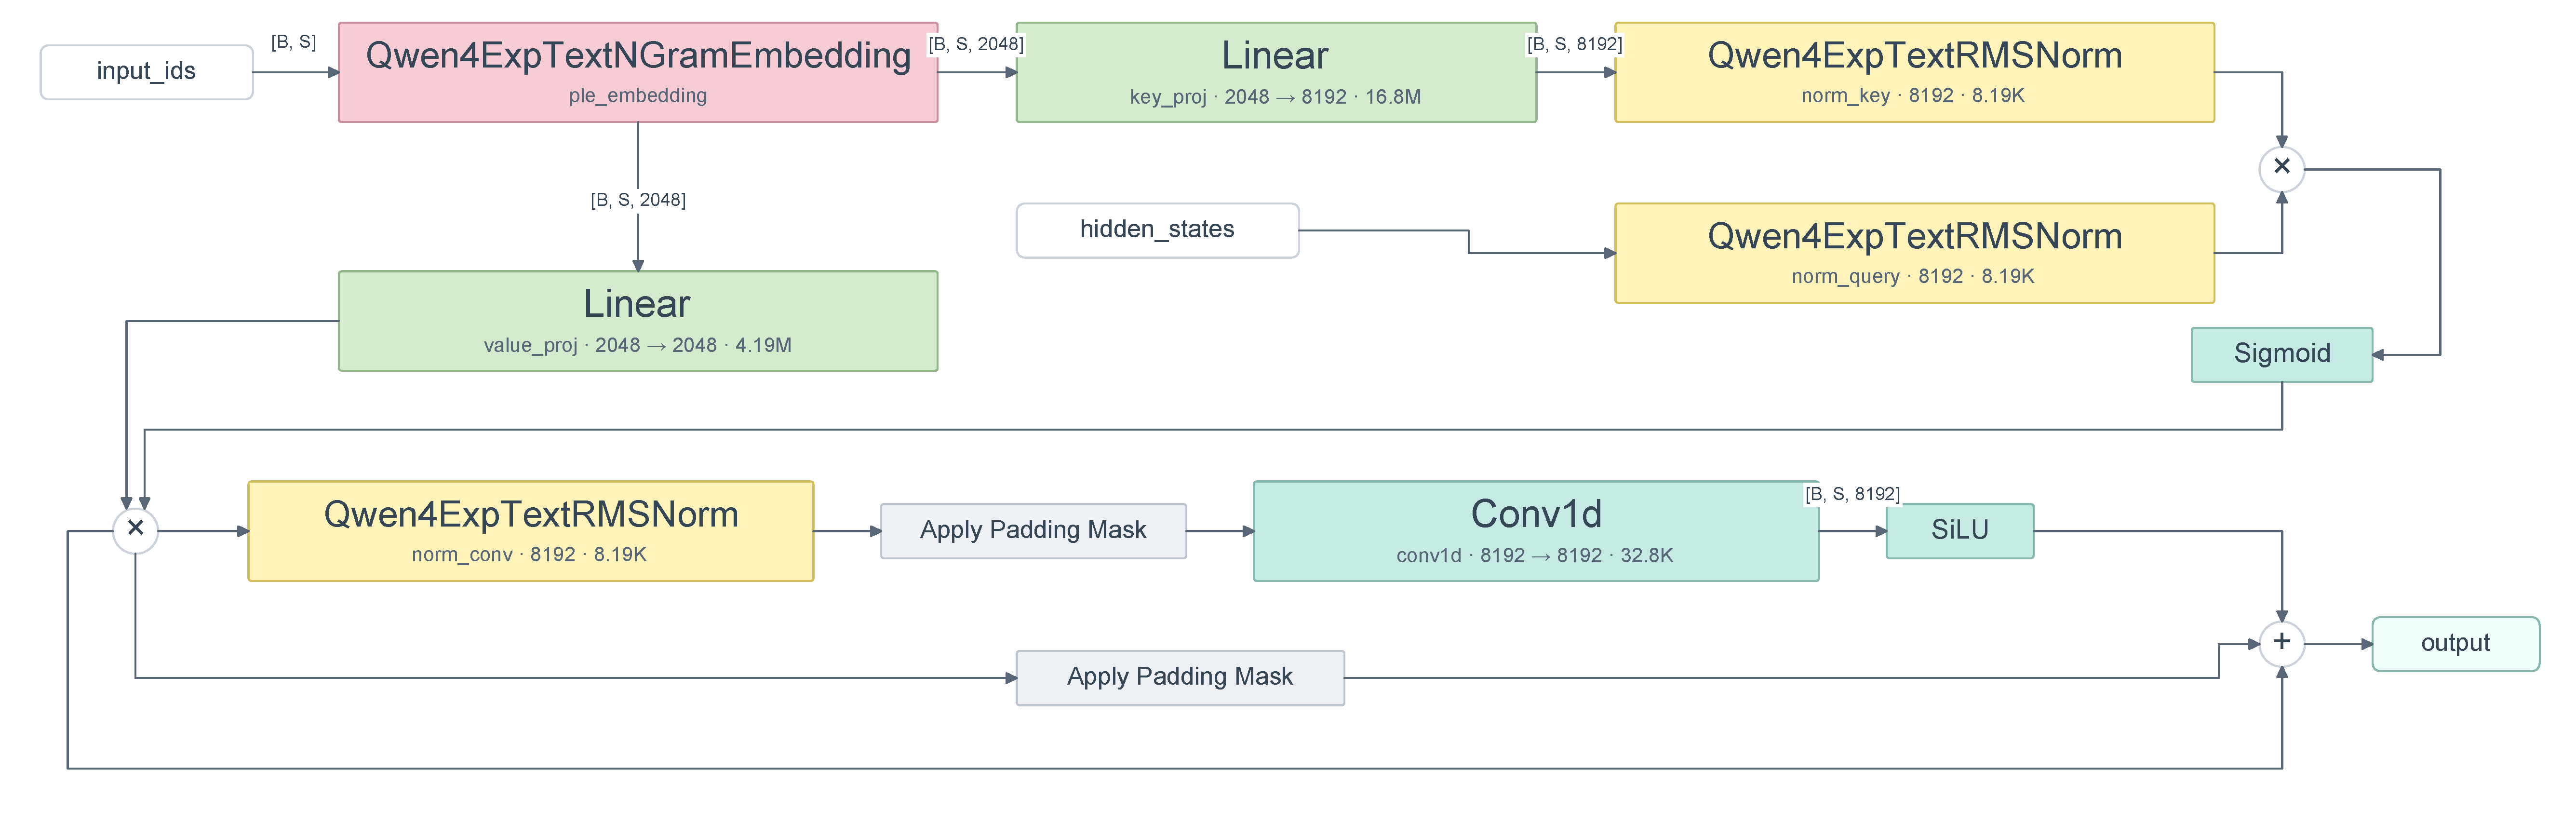
\includegraphics[width=\linewidth]{images/Qwen3.8-Flash-Next/redraw/exports/fig-309.pdf}\par
{\small Qwen4ExpTextPLELayer\par}
\vspace{0.6em}
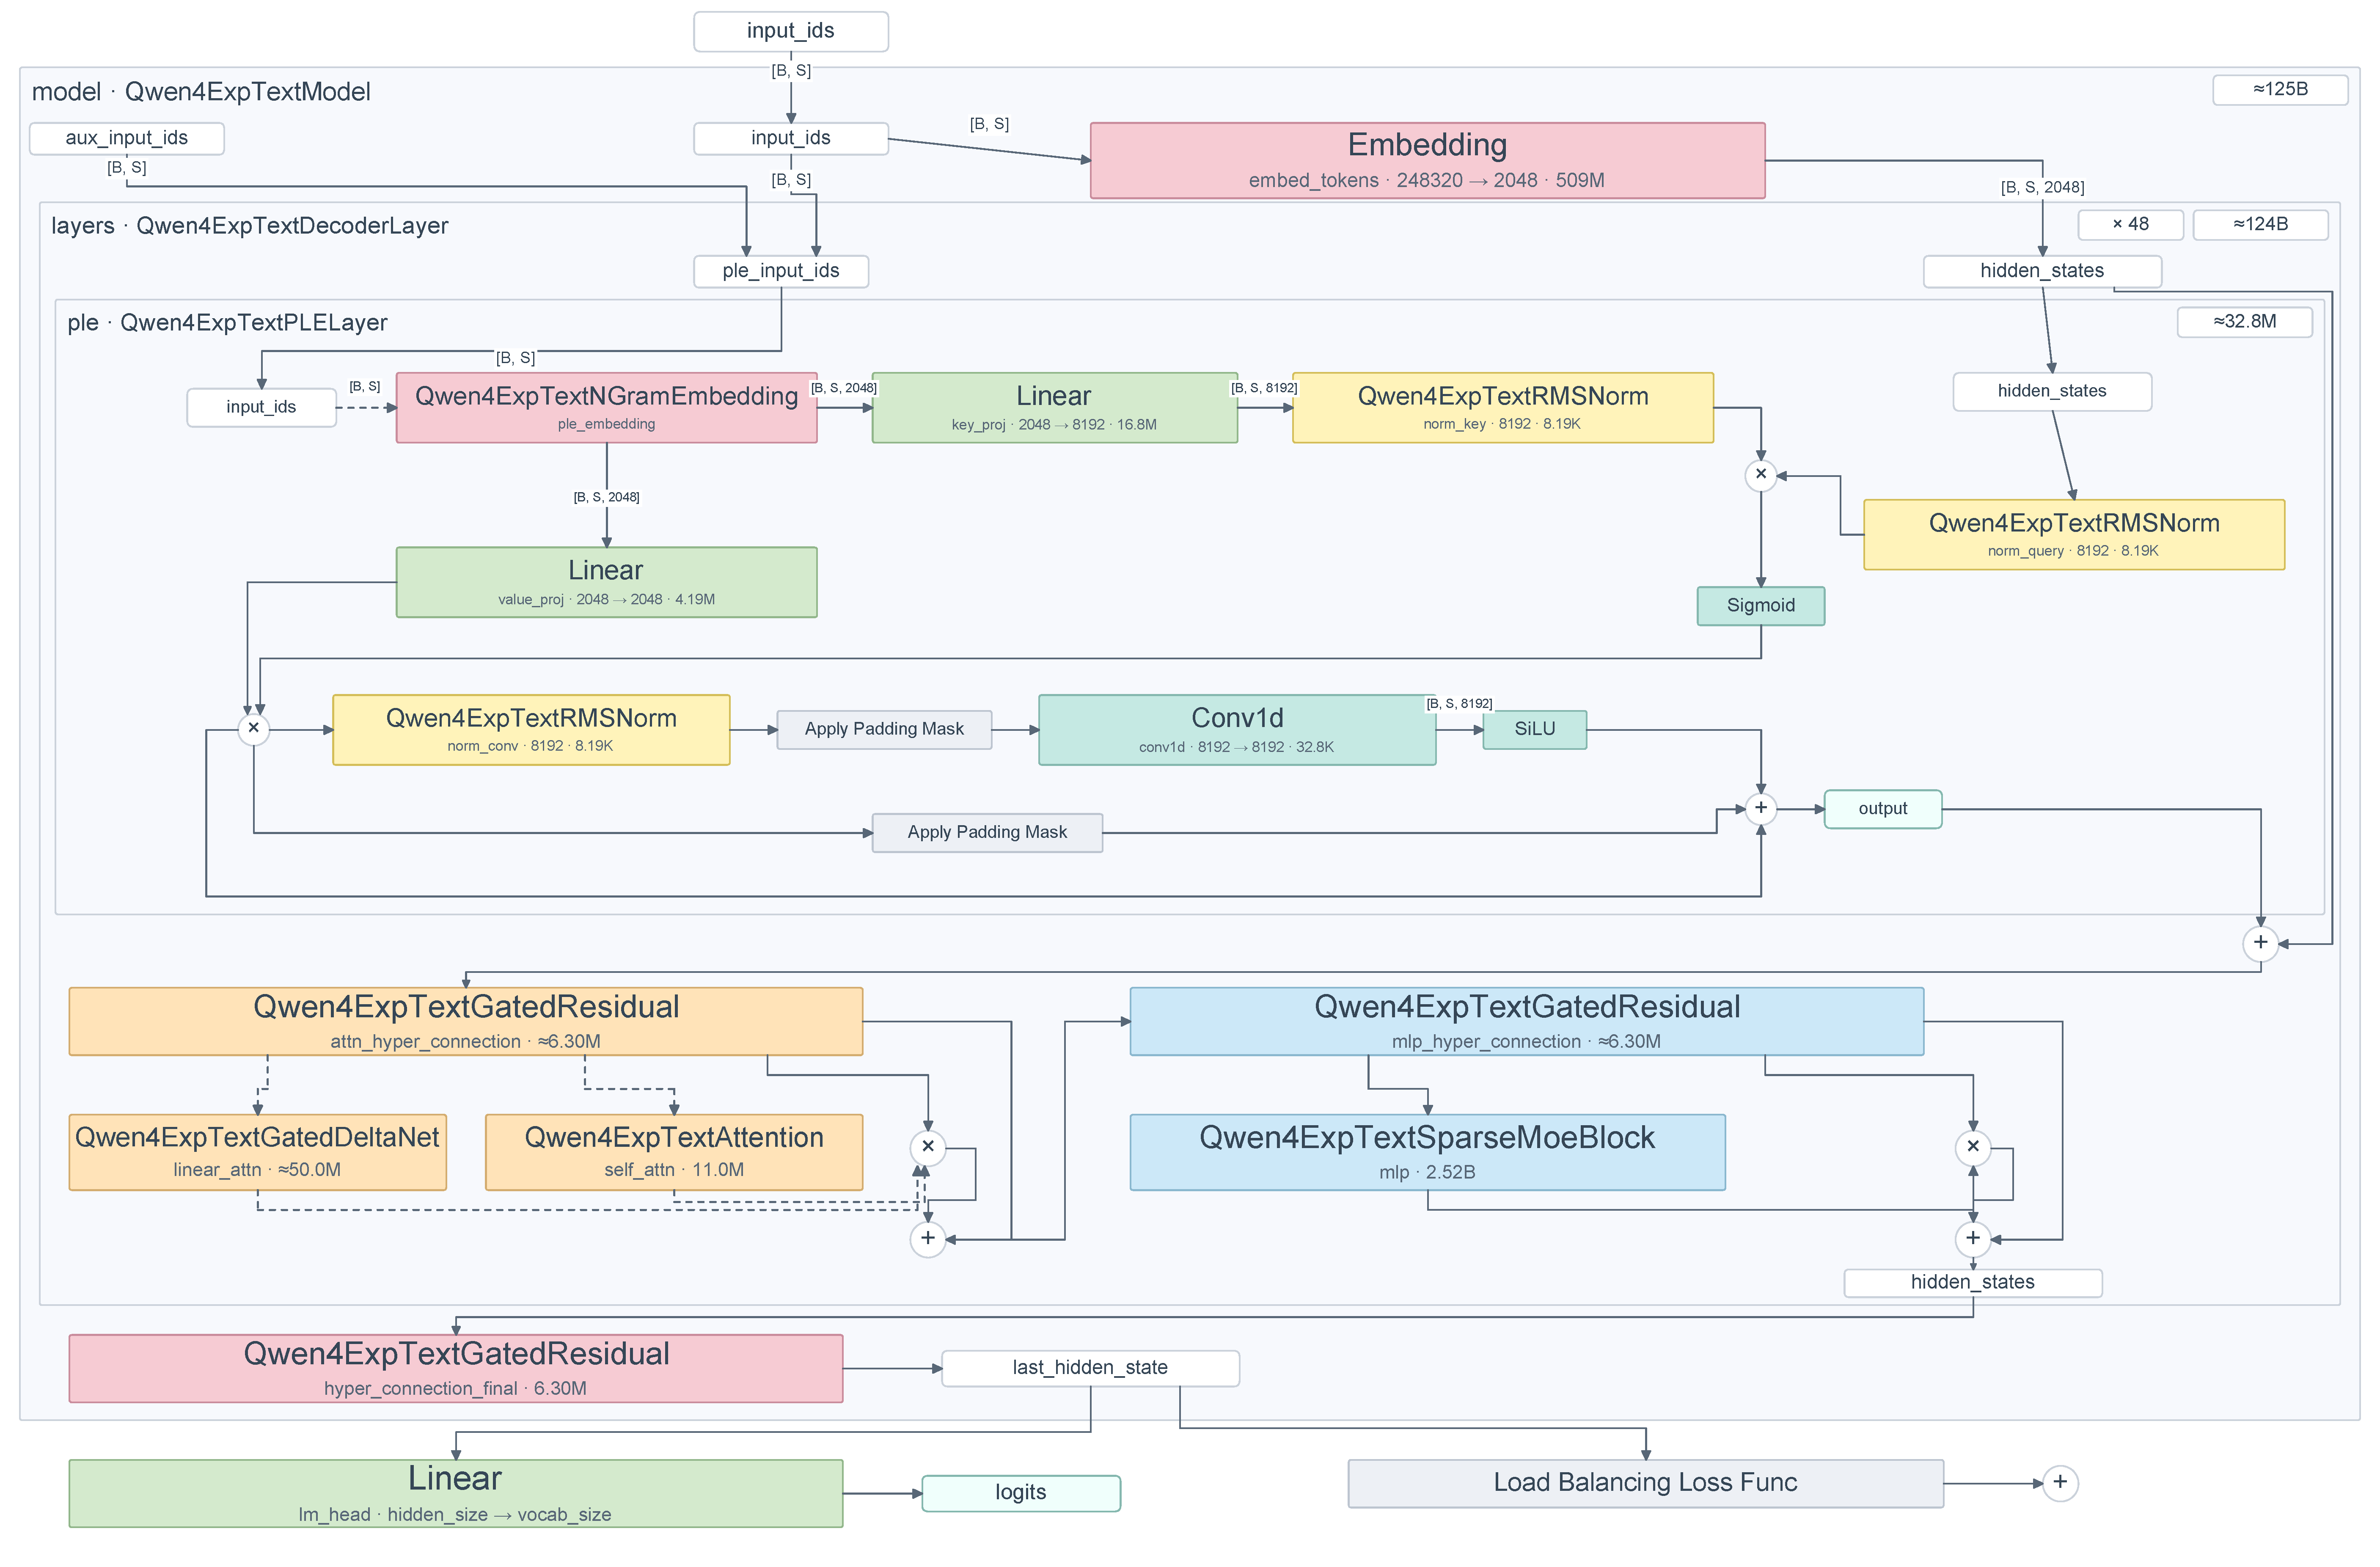
\includegraphics[width=\linewidth]{images/Qwen3.8-Flash-Next/redraw/exports/fig-311.pdf}\par
{\small Qwen4ExpTextPLELayer 在 Qwen-3.8-next 的位置\par}
\end{minipage}
\end{center}
\textcolor{feishuRed}{\textbf{从宏观上看 N-gram Embedding 模块就是 Engram}}：主体逻辑都是用后缀 n-gram 做 key、多头哈希查表、再与当前隐状态门控融合。

\begin{feishubox}{callGreen}{🧭}
\textcolor{feishuRed}{\textbf{Engram：在标准的 Transformer 主干结构上增加 Engram 条件记忆模块，}}通过残差连接将Engram串联到 Transformer-Block主干网络：$\mathbf H^{(\ell)}\leftarrow\mathbf H^{(\ell)}+\mathbf Y$，\textcolor{feishuRed}{注意模型结构中只有部分 Transformer-Block 增加 Engram 模块。}

增加 Engram 模块后，在架构上静态模式存储（Engram）与动态计算（Attention、FFN）分离。

\textcolor{feishuRed}{\textbf{新的模型结构处理每一个位置}}$t$\textcolor{feishuRed}{\textbf{的 token 方法分为两个阶段：}}给定一个输入序列 $X=(x_1,\ldots,x_T)$ 以及第 $\ell$ 层的隐藏状态 $\mathbf H^{(\ell)}\in\mathbb R^{T\times d}$，Engram\textcolor{feishuRed}{\textbf{ }}模块通过\textcolor{feishuRed}{检索和融合两个阶段}处理每个位置 $t$的特征：

\begin{itemize}
\item \textbf{检索：}提取并压缩后缀 $N$-gram，通过多头哈希检索静态嵌入向量（记忆向量）。
\item \textbf{融合：}检索到的静态嵌入向量与当前隐藏状态进行 CrossAttn 动态融合，并通过一个轻量卷积扩展表达能力。
\end{itemize}
\end{feishubox}
我们直接复用 \href{https://my.feishu.cn/wiki/JwXTw0oUeimyoBk2QIgcSfBfn9g}{Engram：Conditional Memory via Scalable Lookup} 中的符号表示：$g_{t,n}$ 是位置 $t$ 结尾的 n-gram，$\phi_{n,k}$ 是第 $n$ 阶第 $k$ 个头的哈希函数，$\mathbf E_{n,k}$ 是对应的嵌入表，$\mathbf e_t$ 是拼起来的记忆向量。

检索阶段要解决的问题：这步需要用n-gram组合进行记忆向量召回，但是直接参数化所有可能的n-gram组合（如3-gram）导致参数爆炸。

\textbf{解决方法}：

\begin{enumerate}
\item[\textcolor{feishuBlue}{1.}] \textbf{哈希降维（解决组合参数爆炸问题）}：对 n-gram token ids 序列$g_{t,n}$，通过哈希函数$\phi_{n,k}$映射到固定维度的索引$z_{t,n,k}$，从嵌入表$\mathbf E_{n,k}$中检索向量$\mathbf e_{t,n,k}$：
\begin{itemize}
\item 计算 n-gram 的哈希值：$z_{t,n,k}\triangleq\phi_{n,k}(g_{t,n})$
\item 在嵌入表（记忆）中检索：$\mathbf e_{t,n,k}=\mathbf E_{n,k}[z_{t,n,k}]$
\item 不同n-gram的记忆向量进行concat：$\mathbf e_t\triangleq\mathop{\Vert}_{n=2}^{N}\mathop{\Vert}_{k=1}^{K}\mathbf e_{t,n,k}$
\end{itemize}
\begin{feishuquote}
$g_{t,n}$ 是以位置 $t$ 结尾、长度为 $n$ 的 token 序列（n-gram）。$N=3$，所以 $n$ 取 2 和 3 两阶。

$K=8$ 是每一阶的 head 数，总头数 $(N-1)\times K=16$。

$\phi_{n,k}$ 是哈希函数：各位置 token id 乘上该位置的乘子后逐位异或（multiplicative-XOR），与 Engram 相同。

$\mathbf e_{t,n,k}\in\mathbb R^{160}$，16 个 head 拼接起来 $\mathbf e_t\in\mathbb R^{2560}$，等于主干网络维度 $C$。

\end{feishuquote}
\item[\textcolor{feishuBlue}{2.}] \textbf{多头机制（解决哈希冲突问题）}：对每个n-gram阶数$n$，使用 k 个独立哈希头（\textcolor{feishuRed}{每个头使用相同的哈希函数和不同嵌入表}），降低哈希碰撞的影响。
\end{enumerate}
相比 \href{https://my.feishu.cn/wiki/JwXTw0oUeimyoBk2QIgcSfBfn9g}{Engram：Conditional Memory via Scalable Lookup}，Qwen-3.8-Next N-gram Embedding 实现上的区别：

\begin{tcbraster}[raster columns=2,raster equal height=rows,raster column skip=9pt,raster row skip=8pt,raster left skip=0pt,raster right skip=0pt]
\begin{tcolorbox}[enhanced,blankest,valign=top]
\begin{itemize}
\item $g_{t,n}$ 直接用原始 token id，不做归一化压缩，相比之下 Engram 需要做\href{https://scnajei2ds6y.feishu.cn/wiki/HXOAwYUENiioNGkwmu9c5sE8nBf\#share-PuXYd5HQCo3SVXxqbQKcIeo2nRb}{分词器压缩（Tokenizer Compression）}。
\item 每个头的表长 $|\mathbf E_{n,k}|$ 取各自不同的质数，降低两个 ngram 不会在 8 个头上 hash 碰撞。
\item Qwen 只在第二层上使用 N-gram Embedding（{\setlength{\fboxsep}{0pt}\colorbox{inlinebg}{\strut\ttfamily ple}\colorbox{inlinebg}{\strut\ttfamily \_}\allowbreak{}\colorbox{inlinebg}{\strut\ttfamily layer}\colorbox{inlinebg}{\strut\ttfamily \_}\allowbreak{}\colorbox{inlinebg}{\strut\ttfamily ids:} \colorbox{inlinebg}{\strut\ttfamily [2]}}）。选第 2 层的理由不在表征上，主要是考虑用第一层的计算时间掩盖主机内存的预取延迟。论文：{\setlength{\fboxsep}{0pt}\colorbox{inlinebg}{\strut\ttfamily allowing} \colorbox{inlinebg}{\strut\ttfamily host-memory} \colorbox{inlinebg}{\strut\ttfamily prefetching} \colorbox{inlinebg}{\strut\ttfamily to} \colorbox{inlinebg}{\strut\ttfamily overlap} \colorbox{inlinebg}{\strut\ttfamily with} \colorbox{inlinebg}{\strut\ttfamily the} \colorbox{inlinebg}{\strut\ttfamily computation} \colorbox{inlinebg}{\strut\ttfamily of} \colorbox{inlinebg}{\strut\ttfamily the} \colorbox{inlinebg}{\strut\ttfamily first} \colorbox{inlinebg}{\strut\ttfamily layer}}。
\item 51B 的 Embedding Table 放在 host 内存。$z_{t,n,k}$ 只由输入 token 算出、与模型状态无关，下一步要查哪几行可以提前算出来，于是 $\mathbf E_{n,k}$ 可以留在主机内存里异步预取。
\end{itemize}
\end{tcolorbox}
\begin{tcolorbox}[enhanced,blankest,valign=top]
\begin{center}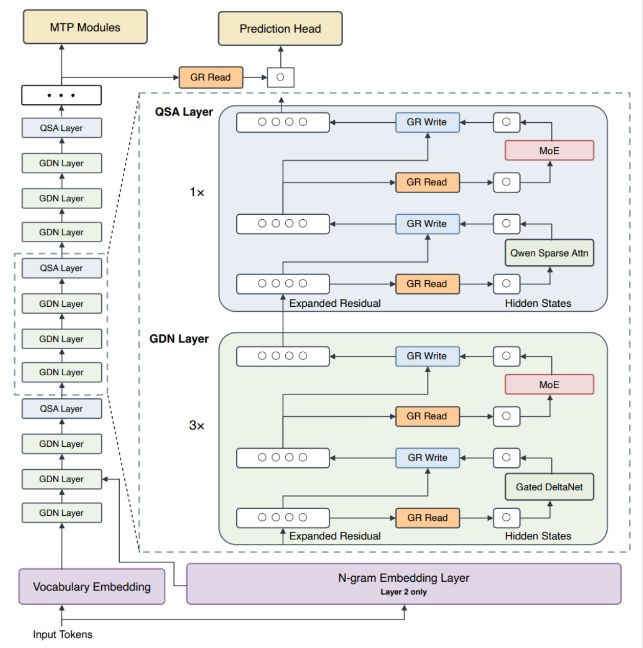
\includegraphics[width=\linewidth,height=.60\textheight,keepaspectratio]{images/Qwen3.8-Flash-Next/fig-331.png}\par{\small Qwen-3.8-next 架构\par}\end{center}
\end{tcolorbox}
\end{tcbraster}
还有一个需要关注的区别：Engram 的融合是在单条残差流上加：$\mathbf H^{(\ell)}\leftarrow\mathbf H^{(\ell)}+\mathbf Y$。Qwen 因为 GR 把残差流加宽成了 $n$ 条，因此需要融合方法端改动：key 投到 $nC$ 维、$n$ 条流各一份。value 只有 $C$ 维、$n$ 条流共用。

解释：每条流各自判断是否写入这条记忆，写入的内容却是同一份。相比之下 Engram 是单流，不存在这个区分。

\begin{center}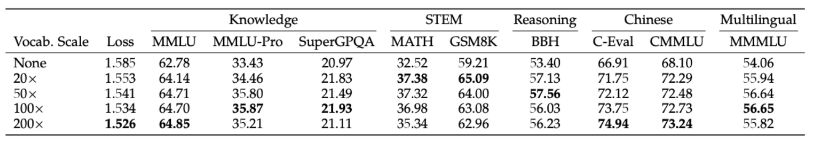
\includegraphics[width=\linewidth,height=.72\textheight,keepaspectratio]{images/Qwen3.8-Flash-Next/fig-196.png}\end{center}
固定预算、把 n-gram 词表从 20 倍缩放到 200 倍基础词表大小：loss 随词表单调下降，下游任务表现不一定变好，MATH 在 20 倍就到达最优，BBH 在 50 倍到达最优，只有中文的 C-Eval 与 CMMLU 随词表一致上升。这个在\href{https://my.feishu.cn/wiki/JwXTw0oUeimyoBk2QIgcSfBfn9g}{Engram：Conditional Memory via Scalable Lookup}实验中也有体现。


\par\vspace{0.95em}\noindent{\zihao{3}\bfseries \textcolor{feishuBlue}{1.5} Vision Encoder}\par\vspace{0.28em}
\par\vspace{0.75em}\noindent{\zihao{4}\bfseries \colorbox{headingGreen}{\parbox{\dimexpr\linewidth-2\fboxsep\relax}{\textcolor{feishuBlue}{1.5.1} Positional Embedding}}}\par\vspace{0.28em}
\begin{tcbraster}[raster columns=3,raster equal height=rows,raster column skip=9pt,raster row skip=8pt,raster left skip=0pt,raster right skip=0pt]
\begin{tcolorbox}[enhanced,blankest,valign=top]
\href{https://scnajei2ds6y.feishu.cn/wiki/IBFPwd8kpiW94gkOgCIcTnDZnnh}{Qwen3-VL}以来的 Qwen 视觉语言模型（VLM），在 Vision Encoder 同时有绝对位置编码、2D RoPE 两套位置编码生效：

\begin{itemize}
\item 绝对位置只在作用在进入第一层之前。绝对位置表给出的是一张全局的、随分辨率插值伸缩的坐标图，只作用于输入。本质就是最原始的\href{https://scnajei2ds6y.feishu.cn/wiki/O2arwxGNXi6KrckUG1dcGcbrnWd}{ViT的位置编码}。
\item 2D RoPE 则作用在每一个 ViT 层的注意力。RoPE 给出的是每一层注意力内部的相对位移，只作用于 q 与 k 的内积。2D-RoPE 不再重复叙述，具体可以参考：\href{https://scnajei2ds6y.feishu.cn/wiki/BHUIwyfVUizmwQkKQPFceqJrnEe}{2D-RoPE}。
\end{itemize}
\end{tcolorbox}
\begin{tcolorbox}[enhanced,blankest,valign=top]
\begin{center}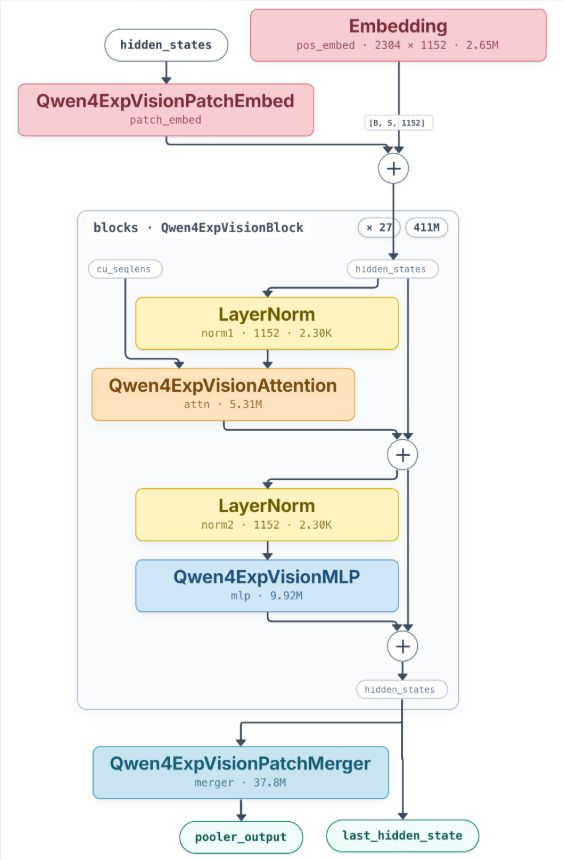
\includegraphics[width=\linewidth,height=.60\textheight,keepaspectratio]{images/Qwen3.8-Flash-Next/fig-337.png}\par{\small Qwen3.8 Vision Model\par}\end{center}
\end{tcolorbox}
\begin{tcolorbox}[enhanced,blankest,valign=top]
\begin{center}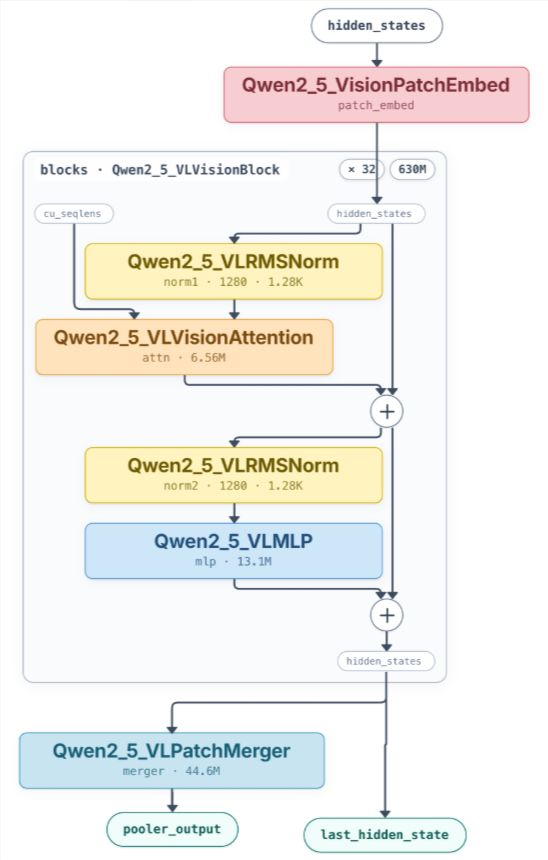
\includegraphics[width=\linewidth,height=.60\textheight,keepaspectratio]{images/Qwen3.8-Flash-Next/fig-339.png}\par{\small Qwen2.5 Vision Model\par}\end{center}
\end{tcolorbox}
\end{tcbraster}
绝对位置编码 {\setlength{\fboxsep}{0pt}\colorbox{inlinebg}{\strut\ttfamily nn.Embedding(2304,} \colorbox{inlinebg}{\strut\ttfamily 1152)}} 本质是训练阶段可学习的 Embedding 表，$2304=48^2$ 对应固定的 48$\times$48 网格。对任意分辨率输入，先用双线性插值把网格重采样到实际的 patch 网格上，再与 patch 嵌入相加：


\par\vspace{0.75em}\noindent{\zihao{4}\bfseries \colorbox{headingGreen}{\parbox{\dimexpr\linewidth-2\fboxsep\relax}{\textcolor{feishuBlue}{1.5.2} PatchMerger}}}\par\vspace{0.28em}
{\setlength{\fboxsep}{0pt}\colorbox{inlinebg}{\strut\ttfamily Qwen4ExpVisionPatchMerger}} 把 2$\times$2 的空间邻域拼成一个 token 再投影到主干宽度：

\begin{center}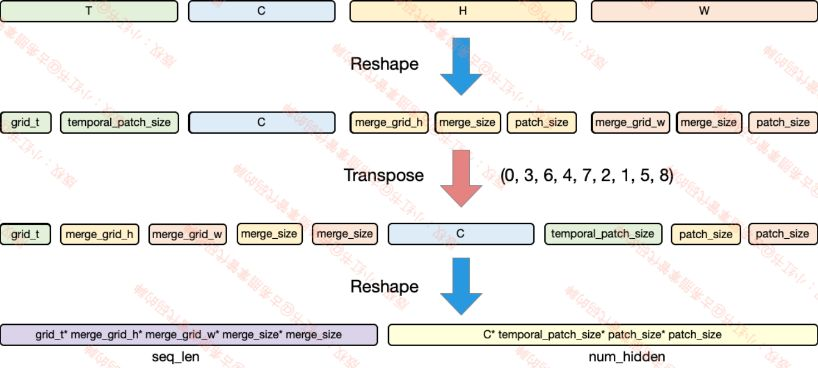
\includegraphics[width=\linewidth,height=.72\textheight,keepaspectratio]{images/Qwen3.8-Flash-Next/fig-207.png}\end{center}
此外 {\setlength{\fboxsep}{0pt}\colorbox{inlinebg}{\strut\ttfamily deepstack}\colorbox{inlinebg}{\strut\ttfamily \_}\allowbreak{}\colorbox{inlinebg}{\strut\ttfamily visual}\colorbox{inlinebg}{\strut\ttfamily \_}\allowbreak{}\colorbox{inlinebg}{\strut\ttfamily indexes}} 取空列表，这个是 \href{https://scnajei2ds6y.feishu.cn/wiki/IBFPwd8kpiW94gkOgCIcTnDZnnh}{Qwen3-VL} 用 DeepStack 把 ViT 若干中间层的特征分别注入 LLM 的前几层，这里\textcolor{feishuRed}{\textbf{退回到只取最后一层、单点注入}}，即不启用 DeepStack。

\begin{feishuquote}
拓展阅读：\href{https://scnajei2ds6y.feishu.cn/wiki/D0tPwY7uZijRxLkQ0pDc9R0cn6g}{PatchMerger 是如何合并 2x2 的 Patch 的？}

\end{feishuquote}

\par\vspace{0.75em}\noindent{\zihao{4}\bfseries \colorbox{headingGreen}{\parbox{\dimexpr\linewidth-2\fboxsep\relax}{\textcolor{feishuBlue}{1.5.3} 其他配置细节}}}\par\vspace{0.28em}
\begin{itemize}
\item \textbf{Interleaved MRoPE：}主干的 RoPE 在多模态下是 M-RoPE，把位置拆成时间、高、宽三个通道交错，具体参考 \href{https://scnajei2ds6y.feishu.cn/wiki/Tyyvw5AmBivxTDkmkMZcT7UmnOc?renamingWikiNode=false}{字节面试官：Interleaved MRoPE 相比 MRoPE 改进？ }。
\end{itemize}
\begin{tcbraster}[raster columns=2,raster equal height=rows,raster column skip=9pt,raster row skip=8pt,raster left skip=0pt,raster right skip=0pt]
\begin{tcolorbox}[enhanced,blankest,valign=top]
\begin{center}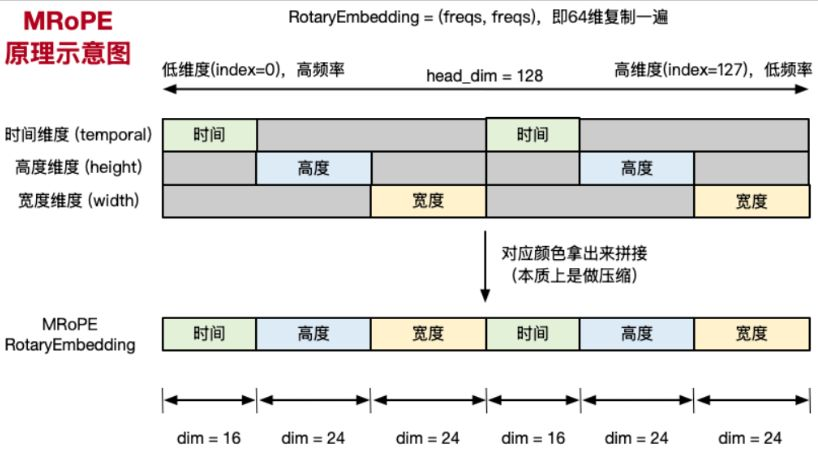
\includegraphics[width=\linewidth,height=.60\textheight,keepaspectratio]{images/Qwen3.8-Flash-Next/fig-342.png}\end{center}
\end{tcolorbox}
\begin{tcolorbox}[enhanced,blankest,valign=top]
\begin{center}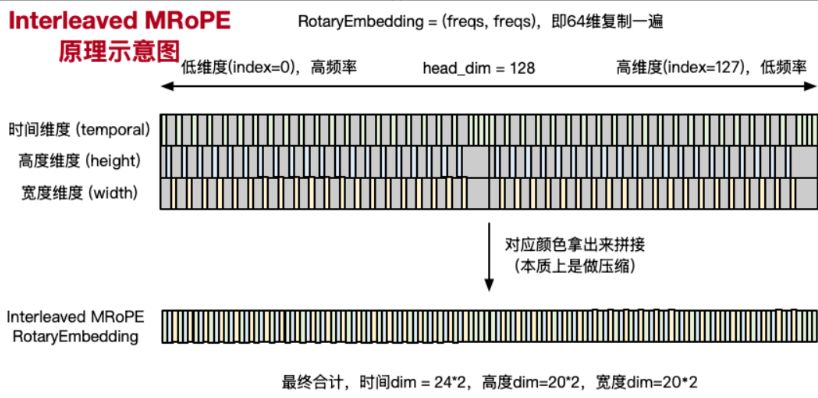
\includegraphics[width=\linewidth,height=.60\textheight,keepaspectratio]{images/Qwen3.8-Flash-Next/fig-344.png}\end{center}
\end{tcolorbox}
\end{tcbraster}
\begin{itemize}
\item \textbf{图像 token 不进 n-gram 表：}{\setlength{\fboxsep}{0pt}\colorbox{inlinebg}{\strut\ttfamily ple}\colorbox{inlinebg}{\strut\ttfamily \_}\allowbreak{}\colorbox{inlinebg}{\strut\ttfamily input}\colorbox{inlinebg}{\strut\ttfamily \_}\allowbreak{}\colorbox{inlinebg}{\strut\ttfamily ids}} 是在视觉特征写入之前取的，51B 的 n-gram table 对图像内容不提供任何检索能力，它只对文本 token 起作用：
\end{itemize}

\par\vspace{0.95em}\noindent{\zihao{3}\bfseries \textcolor{feishuBlue}{1.6} MoE}\par\vspace{0.28em}
MoE 设置 512 个路由专家、每 token 激活 10 个（Top=10），带门控共享专家 1 个：

\begin{enumerate}
\item[\textcolor{feishuBlue}{1.}] \textcolor{feishuRed}{\textbf{激活门控是 softmax 而非 sigmoid，并且没有 loss-free balance 的偏置项。}} 这一项主要对比的是同期 \href{https://scnajei2ds6y.feishu.cn/wiki/KOBowKTbgiv6ewkHhEBc6qCNnPe}{GLM-5.3-Flash}、DeepSeek V4 的 sigmoid 门控 + 无辅助损失偏置。
\item[\textcolor{feishuBlue}{2.}] \textcolor{feishuRed}{\textbf{共享专家先经过一个逐 token 的标量 sigmoid 门再相加。}}{\setlength{\fboxsep}{0pt}\colorbox{inlinebg}{\strut\ttfamily shared}\colorbox{inlinebg}{\strut\ttfamily \_}\allowbreak{}\colorbox{inlinebg}{\strut\ttfamily expert}\colorbox{inlinebg}{\strut\ttfamily \_}\allowbreak{}\colorbox{inlinebg}{\strut\ttfamily gate}} 是 {\setlength{\fboxsep}{0pt}\colorbox{inlinebg}{\strut\ttfamily Linear(hidden}\colorbox{inlinebg}{\strut\ttfamily \_}\allowbreak{}\colorbox{inlinebg}{\strut\ttfamily size,} \colorbox{inlinebg}{\strut\ttfamily 1)}}，由每个 token 自行决定共享专家输出的权重。
\end{enumerate}

\par\vspace{1.15em}\noindent{\zihao{-2}\bfseries \colorbox{headingPink}{\parbox{\dimexpr\linewidth-2\fboxsep\relax}{\textcolor{feishuBlue}{2.} Muon\textbf{ 优化器}}}}\par\vspace{0.28em}
\begin{feishuquote}
拓展阅读：\href{https://my.feishu.cn/wiki/Hcj2wGTJEiohTikkdEKc7H4Nnlb}{Muon 优化器}

\end{feishuquote}
\textbf{使用 Muon 的权重：}注意力的 q/k/v 与输出投影、GDN 的输入输出投影、路由专家与共享专家的 fc1/fc2、n-gram 嵌入层的 key/value 投影。

\textbf{使用 AdamW 上的权重：}输入嵌入、输出头、MoE 路由器、GR 的低秩投影，n-gram 嵌入表使用关闭 weight decay 的 Adam。

\begin{itemize}
\item 路由器保留 AdamW 的理由：Muon 加剧早期训练波动并使路由器失稳，即便中后期再启用也没有显著收益。
\item GR 的低秩投影同样更适合 AdamW，原因在于其形状极度细长。
\item 融合参数必须先切分再正交化：Megatron-LM 里 qkv 投影、SwiGLU 的 fc1、GDN 输入投影都按输出维融合成一个矩阵，语义上却是若干独立线性算子的拼接。直接正交化会把互不相关子块的奇异方向混合。因此在正交化前先切分梯度缓冲、逐块执行 NS 迭代、再聚回原 tensor 布局。
\end{itemize}
\href{https://my.feishu.cn/wiki/UsuawakRYiqacxkD9vxcKzylnoe}{DeepSeek V4} 在使用 Muon 优化器上同样选择隔离部分参数使用 AdamW：

\begin{center}\renewcommand{\arraystretch}{1.3}\begin{tabularx}{\linewidth}{|>{\raggedright\arraybackslash}X|>{\raggedright\arraybackslash}X|}
\hline
\rowcolor{tableHead}
\textbf{模块} & 优化器\\\hline
\textbf{Embedding} & AdamW\\\hline
\textbf{Prediction head} & AdamW\\\hline
\textbf{mHC 的静态 bias }$\mathbf S_l$\textbf{、gating factor }$\alpha_l$ & AdamW\\\hline
\textbf{RMSNorm} & AdamW\\\hline
\textbf{其他所有参数（attention, MoE expert, mHC等）} & \textbf{Muon}\\\hline
\end{tabularx}\end{center}
\begin{itemize}
\item embedding / head 稀疏更新（每次只更新 batch 里出现的 token 行），走 AdamW。
\item RMSNorm、mHC 是 1D 向量，Muon 对标量/向量没有意义。
\end{itemize}

\Needspace{.50\textheight}\par\vspace{1.15em}\noindent{\zihao{-2}\bfseries \colorbox{headingPink}{\parbox{\dimexpr\linewidth-2\fboxsep\relax}{\textcolor{feishuBlue}{3.} 实验}}}\par\vspace{0.28em}
\begin{center}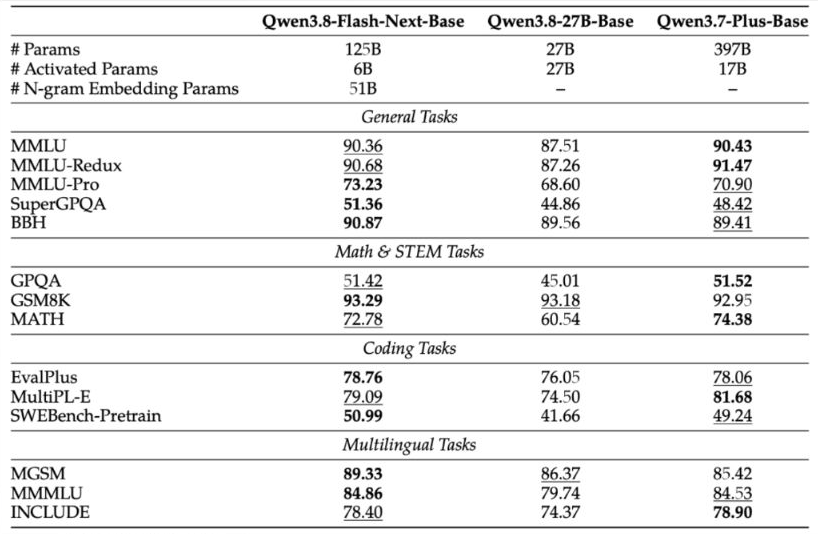
\includegraphics[width=.92\linewidth,height=.72\textheight,keepaspectratio]{images/Qwen3.8-Flash-Next/fig-237.png}\end{center}
对比上一代 397B-A17B，激活参数只有三分之一，Qwen3.8-Flash-Next 优势主要体现在效率而非绝对能力。因此 Qwen3.8-Flash-Next 更像是 Qwen-4 系列的架构 Scaling 探索而不是完整 Scaling 训练后的产物。对比同期模型，Qwen3.8-Flash-Next 和 \href{https://scnajei2ds6y.feishu.cn/wiki/Ax5kwJIWRiF7lSkliAucQYwBnHf}{Kimi K3}、\href{https://scnajei2ds6y.feishu.cn/wiki/KOBowKTbgiv6ewkHhEBc6qCNnPe}{GLM-5.3-Flash}、\href{https://my.feishu.cn/wiki/UsuawakRYiqacxkD9vxcKzylnoe}{DeepSeek V4} 有很多架构设计上的趋同，下篇拆解。

\end{document}
